\documentclass{article}

\usepackage[utf8]{inputenc}

\usepackage{graphicx}
\usepackage{subcaption}
\usepackage{mathtools}
\usepackage{wrapfig}
\usepackage{graphicx}
\usepackage{subcaption}
\usepackage{mathtools}
\usepackage{wrapfig}
\usepackage{float}
\usepackage{gensymb}
\usepackage{caption}
\usepackage{geometry}
\usepackage{cite}

\DeclareMathOperator{\sech}{sech}
\DeclareMathOperator{\Tr}{Tr}

\usepackage{listings}
\usepackage{color}

\definecolor{codegreen}{rgb}{0,0.6,0}
\definecolor{codegray}{rgb}{0.5,0.5,0.5}
\definecolor{codepurple}{rgb}{0.58,0,0.82}
\definecolor{backcolour}{rgb}{0.95,0.95,0.92}
 
\lstdefinestyle{mystyle}{
    backgroundcolor=\color{backcolour},   
    commentstyle=\color{codegreen},
    keywordstyle=\color{magenta},
    numberstyle=\tiny\color{codegray},
    stringstyle=\color{codepurple},
    basicstyle=\footnotesize,
    breakatwhitespace=false,         
    breaklines=true,                 
    captionpos=b,                    
    keepspaces=true,                 
    numbers=left,                    
    numbersep=5pt,                  
    showspaces=false,                
    showstringspaces=false,
    showtabs=false,                  
    tabsize=2
}

%\usepackage{minted}
%\begin{minted}{haskell}
 
\lstset{style=mystyle}





\makeatletter
\renewcommand\paragraph{\@startsection{paragraph}{4}{\z@}%
	{-2.5ex\@plus -1ex \@minus -.25ex}%
	{1.25ex \@plus .25ex}%
	{\normalfont\normalsize\bfseries}}
\makeatother
\setcounter{secnumdepth}{4} % how many sectioning levels to assign numbers to
\setcounter{tocdepth}{4}    % how many sectioning levels to show in ToC in preamble





\geometry
{
  %body={6.5in, 8.5in},
  left=1.0in,
  top=1.25in
}

\setlength{\parindent}{10ex}









%\begin{figure}[H]
%	\centering
%	\includegraphics[scale=0.2]{rhul_logo}
%\end{figure}








%chris help

%how should I split my code as its to long

% in section 5.5 your code has thd3.hd, why is this hd there? you have already headed the inputs list hence returning a list of the wrappers for that time step. So why head again? is this becasue each set of messages are in their own list?


%how does . work as i cant get it to work thd3.hd






%increase margin size! 
%abm dynamic, and RR analytic (not top down and bottom up) well abm are bottom up but rr may not be top down 
\begin{document} 
\title{Translating from First Order Recurrence Relations to an Agent-Based Representation} 
\author{Leo Carlos-Sandberg\\
Supervisor: Dr Christopher D. Clack} 
\maketitle 

\begin{abstract}
\noindent {\it 
%move two-views to later one, (if you say we will use two views (no -), two-views approach)
%start talking about, the ability to translate from one view point to another to demsotrate their equilvnece
%and why are we translating  
This paper investigates a method of describing interacting systems from two opposing view points, recurrence relations and agent-based models. These two methods take fundamentally different approaches with recurrence relations being top-down, and agent-based models being bottom-up.\\
Connecting these two methods allows for a more complete investigation of emergent behaviour occurring within interacting systems. Agent-based models offer an attractive way of analysing emergent behaviour, with the ability to investigate individual interactions as message passing throughout a simulation. Agent-based models however tend to be less well understood and accepted by those outside computer science, this is in contrast to recurrence relation which are normally well understood. Creating a correctness preserving link between recurrence relations and agent-based models allows for simulations to be understood in their recurrence relation representation and hence have their agent-based model representation accepted. This is important in fields such as finance as it opens up new tools for economists and regulators to use in understanding emergence in complex markets.\\
This research comprises the definition of a simple recurrence relation language, to define simulations, and the design of a step-by-step process by which a set of recurrence relations defined in this language can be converted into an agent-based model representation, the InterDyne simulator is chosen as a target representation for this transformation. 

}
\end{abstract}




\newpage
\newgeometry{top = 2cm}
\tableofcontents
{\textit{ }}
\restoregeometry
\newpage



%\begin{figure}[H]
%	\centering
%	\includegraphics[scale=0.5]{spin_on_lattice}
%	\caption{\it The two-dimensional Ising model lattice.}
%	\label{fig:spins_on_lattice_demo}
%\end{figure} 

%\begin{equation}
%E = -J\sum_{\langle i,j \rangle}^{N} s_{i}s_{j} - h \sum_{i = 1}^{N} s_{i}.
%\end{equation}

%\label{1d_code}

%~\cite{GouldBook} 
%~\ref{s_the_ising_model} 

%%%%%%%%%%%%%%%%%%%%%%%%%%%%%%%%%%%%%%%%%%%%%%%%%%%%%%%%%%%%%%%%%%%%%%%%%%%%%%%%%%%%%%%%%%%%%%%%%%%%%%%%%%%%%%%%%%
\section{Introduction}
Complex systems have been an area of interest for a long time in many  fields such as physics, biology and chemistry [REFS????]. %get very very old reference to this 
 More recently this is true in the fields of economics and finance [REFS?????], especially as the financial markets have become increasingly automated and interconnected. 
%These systems can exhibit unexpected and hard to predict behaviour, known as emergence, which can some times, have a large impact and damage a system.\\ 
Of particular interest is emergent behaviour in complex systems given by name "".
% not this any more (These systems can exhibit behaviour that is unexpected  and hard to predict, and which can have a large impact and  cause damage. )
%define emergence (very short) from chapter fromm 2005 types and forms of emergence (arxiv preprint nlin/0506028)  
 %hard to predict because it cant be reduced down to the definition of the compent parts 
 %page 3 top in fromm paper 2.1 is a definition (check his references reference all three) 
 
Emergent behaviour can occur in a large number of ways, but more often the behaviour of interest is created over a time period. In general there are two ways of viewing systems in time, these are either continuous (where the system progress through time smoothly) or discrete (where the system takes equal quantised steps through time, with each step advancing the system).

For discrete time systems two particular modelling techniques that can be used are, recurrence relations and agent-based models. %These two methods take fundamentally different views of a system, recurrence relations take a top down view and can be seen as a set of mathematical equations which make calls for the values of each other. Agent-based models take a bottom up approach and model different elements of the system as individual agents which communicate via messages passed between each other.\\
%analytic verses dynamic approaches 

Both of these techniques have been extensively used in the modelling of complex systems, in a larger range of fields [REFS???]. %REFS????
Recurrence relations have a number of advantages such as [REFS???]:
\begin{itemize}
%  \item Being well understood in a large number of fields. 
  \item Giving a formal mathematical definition of the whole system.
  \item Showing an obvious link between equations within the system. 
  \item Giving a static representation of the system.  
\end{itemize}
Agent-based modelling benefits include [REFS???]:
\begin{itemize}
  \item Being able to encode unique agents, with varying levels of complexity.
  \item Giving a dynamic representation of the system's evolution. 
  \item Plainly showing the passing of information between agents.
  \item Easily expandable by adding more agents.  
\end{itemize}          
The ability of agent-based models to track the communication between agents and their bottom up approach makes them particularly adept at analysing emergent behaviour. 

As mentioned there has been a growing interest into complex systems and emergence in finance, a large part of this interest is on regulating these systems to stop the creation of destructive emergent behaviour [REFS????]. This has been especially true when looking at high-frequency trading, which has been accused of causing a number of negative effects within the markets, including flash crashes [REFS???]. 
%This trading takes place at high speeds comparable to the ticks on a computers internal clock, meaning models of this type of trading typically will take a discrete time approach.\\
%just say computer trading is discrete (use chapter for help)

Though both agent-based models and recurrence relations have been used within finance, there is a notable preference among researchers grounded in economics to use recurrence relations.\footnote{This is discussed further in Section~\ref{litreviewofabmrr}.} This preference appears to be caused by agent-based models not resonating with these researchers, 
%leading to them passing over using the models as well as results be other researchers using the models being less widely accepted.\\
%rewrite this sentence break it up

%break this sentence up 
This lack of acceptance presents a problem for work on emergence within the financial system; agent-based models are a strong tool in investigating emergent behaviour, ignoring them seriously limit the ability to research this area, and a large amount of research has already been done in this area using agent-based model, if this work is only accepted by a subsection of the community its impact will be substantially lessened.     

This paper seeks to present a method whereby agent-based models will resonate better with experts such as economists, and with the hope that they will be used more frequently and the research based upon them will be better accepted.   

%be a political, dont get at econmimist at all just talk about the two different models and how 
This raises the question, how can agent-based models be explained to a sceptic in such a way that they will accept them? This papers approach is to connect agent-based models and recurrence relations together, allowing the already accepted recurrence relations to become the formalism of the agent-based model.

For this approach to work, there has to be confidence that the connection between the recurrence relations and agent-based model, has a significance and is correct. Hence the next question is what is a meaningful connect? A correctness preserving transformation was chosen as a connection, allowing the recurrence relations and agent-based model to be two views of the same system, hence giving meaning to the agent-based model of the system in terms of recurrence relations. This approach is coined as the two views.     

This transformation takes a set of recurrence relations and turns them into an agent-based model, this direction has been chosen opposed to the reverse as the aim is to encourage sceptics to engage with agent-based models, so allows them to start with the familiar before the transformation. 

To achieve this transformation from a set of recurrence relations to a agent-based model, a number of conceptual challenges needed to be addressed. These problems are discussed in greater depth in Section~\ref{twoviewsapproach} but including: 
\begin{itemize}
   \item The two paradigms of the models are completely different and opposing. 
   \item How are function calls related to message passing?
   \item How can the idea of agents having a infinite list through out time of their values be derived from the recurrence relations? 
   \item How can the idea of private and public information introduced, and what data should fall into each category? 
   \item How can public broadcast data be introduce, and what data classifies to be treated as such? 
   \item How can time limited information be introduced?
   \item How can name control be introduced in a tangible way into a recurrence relations that have no notion of agents. 
   \item How can output messages containing message information be introduced? 
   \item How can the recurrence relations be split in a way which does not splinter the model? 
   \item How can small, and hence more susceptible to prove of correctness, steps be used to transform the model? 
\end{itemize}
To create a transformation that allows these issues to be overcome and to increase the easy in proofing the correctness of this conversion, a step-by-step approach was taken, where the transformation is done in a series of small correctness preserving steps. 

This papers aim is hence to create the design of each of these steps, in the process of transforming from a set of recurrence relations to an agent-based model.

Creating this transformative method has  two important aspects, increasing the acceptance of agent-based models and creating a model for viewing systems in two perspectives. Increasing the acceptance of agent-based models has a number of benefits including: 
\begin{itemize}
   \item Increasing the use of agent-based models in new research, where their benefits would be more suited. Hence increasing the ease in which emergence can be investigated within the financial system. 
   \item Allow for work already done using agent-based models to be re-evaluated with a greater understanding to the methods used. 
\end{itemize}
The creation of the two views model always a number of unique benefits by providing a new tool for analyse of complex systems: 
 \begin{itemize}
    \item Adds a new technique for viewing and modelling complex systems.
    \item Adds a new tool that can be used for hypotheses formalisation and communication of ideas between researchers. 
    \item Adds a model that is suitable for both static and dynamic analyses. 
 \end{itemize}
The timing of this paper fits with the increased interest in agent-based models within finance, for modelling the complex behaviour of the markets [REFS???????]. %REFS????
This work is designed to be able to support other work done using agent-based models and help further the understanding of agent-based models during this time of interest.

To show a conversion between the two types of models a particular example of each must be chosen, for this paper a custom recurrence relation language was designed to be transformed into the agent-based model known as InterDyne. InterDyne was chosen in particular due to it being designed from the bottom up to model and investigate emergent behaviour within the financial markets, this software was also a convenient choice due to access to the source code and local expertise.   

This papers layout is as follows. First a background is given detailing, emergent behaviour generally and in the financial markets, a description and review of the literature of both recurrence relations and agent-based models, and a in-depth description of InterDyne. Secondly a description and analysis of the problems with agent-based models and how a two-view approach addresses them. Thirdly a description of the design, formal syntax, and use, of the custom recurrence relation language. Fourthly the design and a example of the step-by-step transformation between the two models. Fifthly a validation that the transformed example does indeed represent a InterDyne simulation. Sixthly a test of a number of examples for correctness of functionality. Lastly the paper is concluded and summarised with notes for further work given.     
%This connection between the models is coined as the two-views approach.\\



%regulation is shifting from micro to macro-prudential perspective 
%managing individual risk to managing systemic risk

%USE THIS LINK
%\cite{fallacyofcompostionBook}
%talks about policy due to emergence 
%page 10 
%googled "fallacy of division emergent behaviour"

%no formal description of the problem

%-DEVS model does give you overarching symatic (why is it not approate to model interarction dynamics) 



%Compare difference equations and ABM in intro using the "TO AGENT-BASED SIMULATION FROM SYSTEM DYNAMICS" paper



%in project scope: show some limited implementation. Say initial aim was to design, but not implement the translation steps. However, the project has succeeded in all of the design aims and additionally succeeded in implementing several of the translation steps."


%This makes agent-based models in many cases the most natural way for describing systems composed of ``behavioural'' entities~\cite{techsadsProbsabm}.

%In many cases, ABM is most natural for describing and simulating a system composed of ?behavioral? entities. Whether one is attempting to describe a traffic jam, the stock market, voters, or how an organization works, ABM makes the model seem closer to reality. For example, it is more natural to describe how vehicles move in a lane than to come up with the equations that govern the dynamics of the density of vehicles. Because the density equations result from the behavior of vehicles, the ABM approach will also enable the user to study aggregate properties. (from paper techsadsProbsabm)

%The flexibility of ABM can be observed along multiple dimensions. For example, it is easy to add more agents to an agent-based model. ABM also provides a natural framework for tuning the complexity of the agents: behavior, degree of rationality, ability to learn and evolve, and rules of interactions. Another dimension of flexibility is the ability to change levels of description and aggregation: one can easily play with aggregate agents, subgroups of agents, and single agents, with different levels of description coexisting in a given model. One may want to use ABM when the appropriate level of description or complexity is not known ahead of time and finding it requires some tinkering. (from paper  techsadsProbsabm)

%https://www.ijcsi.org/papers/IJCSI-9-1-3-115-119.pdf



%Abandoning the consistency requirements of RE equilibrium removes the need for solving the models as one single block: in principle AB models can be fully modularised, with endless possibilities for recombination and extension. However, this feature has not been exploited so far. Existing AB models are mostly one-off exercises which do not travel across research groups and whose ?working life? does not usually extend beyond the grant that originated them. Code is not re-used, except possibly by the authors themselves; alternative assumptions are not tested, results are not generalised. In short, knowledge accumulates at a slow pace. The reason for this ?modelling individualism?, as we might call it, is to be searched in the struggle to win the ?modelling race?, in line with existing incentives in terms of (short-term) publications and funding opportunities.
%https://www.nuffield.ox.ac.uk/economics/papers/2015/ABMfuture-v12.pdf

%https://www.ripublication.com/ijaer16/ijaerv11n8_23.pdf (says that abm might be much better then other models)


%Such methods are unfamiliar (or unappealing) to most theorists in the leading research departments and rarely published in the top professional journals. Farmer and Foley attribute this in part to the failure of a particular set of macroeconomic policies, and the resulting ascendancy of the rational expectations hypothesis:


%talk abou tht eneed for the strucutre of recurrance relations needing inital condition and driving expression 



%We want to look at emergent behaviour that comes from interaction dynamics, this relays on viewing the communication between the different components of a system as messaging passing. Agent-based models naturally support this view  making them well suited to analysing emergent behaviour. However most agent-based models do not have a well defined formalisation for the system as a whole, which makes it difficult to perform system wide analytics. 
%recurrence relations naturally suportan system wide analys, but do not support a message passing view of cummonicatiio.
%What we want is a way of viewing a system using both models, hence being able to have the benefits of being able to view the passing of information  this is the two views approach t


%Recently AB models have started to outnumber DE models, but understanding of AB philosophy and methodology is much less widespread than familiarity with DE techniques

%in a number of fields RR are more accepted then abm 
%https://www.ncbi.nlm.nih.gov/pmc/articles/PMC5221574/


%good refrence for comparing agent based models and differenc equations 
%https://pdfs.semanticscholar.org/eff5/1151b58ba82c0bd7c3dd96cc30984067a5a0.pdf


%Today, computer-simulation in the natural sciences and engineering mostly rely on equation-based modeling (e.g. of the dynamics of gases, fluids, or solid bodies). Such an approach would certainly be hard to transfer to the social sciences, as most system behaviors have not been formalized mathematically. A method that seems to be more suited for the computer simulation of socio-economic systems is agent-based modeling (ABM)
%refer
%N. Gilbert, K.G. Troitzsch, Simulation for the Social Scientist. (Open University Press, England, 2005)
%J.M. Epstein, R. Axtell, Growing artificial societies. (Cambridge, MA, 1996)
% J.M. Epstein, Generative Social Science: Studies in Agent-Based Computational Modeling. Princeton Studies in Complexity. (Princeton University Press, Princeton, 2007)



%Parunak et al. (1998) compare agent-based modeling and equation-based modeling. They conclude in part that agent-based modeling is best for spatial problems and individual choices, while equation-based modeling is best for geographically concentrated problems driven by well-defined mathematical rules. Specific equation-based formalisms for analyzing simulations include partial recursive functions, difference equations, and dynamical systems.

%that rr can be used for abm
%Epstein (2007) invalidates the commonly cited dichotomy between computational agent-based models and equation-based models by proving, albeit informally, that all computational agent-based models can be expressed using partial recursive functions. Epstein begins his proof by observing that because any standard computer program is effectively Turing complete, then programs for computational agent-based models must be so as well. Epstein then notes that there is an equivalent partial recursive function for every Turing machine. Therefore, there are sets of partial recursive functions for every computational agent-based model. These partial recursive functions are equations that fully specify any given computational agent-based model. Epstein also uses the partial recursive functions approach to argue informally that computational agent-based models, particularly those in the social sciences, are deductive in nature.


%Taking EBM as formal specification of systems properties has a number of advantages, among which the most important are:
%it means having a formal, higher-level specification for the behavior of the ABM to be designed;
%it allows the precise checking of the behaviors of the implemented ABM, thus guaranteeing a sound basis for the exploration of the features of the system being studied, which the EBM abstracted away;
%the conjunction of the two models is conceptually stronger than the consideration of each model alone, as the EBM may be seen as the modeling of the macro-level of the system being studied, while the ABM may be seen as its implementation at the micro-level.


%%%%%%%%%%%%%%%%%%%%%%%%%%%%%%%%%%%%%%%%%%%%%%%%%%%%%%%%%%%%%%%%%%%%%%%%%%%%%%%%%%%%%%%%%%%%%%%%%%%%%%%%%%%%%%%%%%
\section{Background}
This section covers a description of emergent behaviour, feedback loops as type of this behaviour and their appearance in the financial markets. Recurrence relations and agent-based models are introduced as a method for modelling emegernt behaviour, and they are described. InterDyne is introduced as an example of an agent-based model designed for the financial markets. Its applicability to modelling aspects of the financial market will be discussed and description of its design will also be given.   

%%%%%%%%%%%%%%%%%%%%%%%%%%%%%%%%%%%%%%%%%%%%%%%%%%%%%%%%%
\subsection{Emergent Behaviour}
Emergent behaviour is a term used to describe macro-level behaviour of a system that is not obvious from analysis of the micro-level behaviour of the system, more formally this is behaviour that can not be predicted through analysis of any single component of a system \cite{EB_systemofsystemsGLangford}.

A misunderstanding of emergence can lead to the fallacy of division, this is that a property of the system as a whole most also be a property of an individual component of the system; water for example has a number of properties including being able to be cooled down to become ice and heated to become steam, saying the same must also be true of a molecule of water however is incorrect. This concept continues into economics, being called the fallacy of composition, where what is true for the whole economy my not hold for an individual and vice versa~\cite{fallacyofcompostionBook}.
       
A simple way to demonstrate emergence is in the Game of Life~\cite{gameoflifepage}, which is an example of cellular automaton; this game takes place on an infinite two-dimensional grid in which cells can either be `alive', coloured for example green, or `dead', a different colour usually black. Wether a cell is `alive' or `dead' is based on a set of simple rules:   
\begin{enumerate}
  \item `Alive' cells will transition to be `dead' cells in the next time step if they have few than two `alive' neighbours.
  \item `Alive' cells with two or three `alive' neighbours remain `alive' at the next time step.
  \item `Alive' cells will transition to be 'dead' cells in the next time step if they have more than three `alive' neighbours.
  \item `Dead' cells with exactly three 'alive' neighbours will transition to `alive' at the next time step.
\end{enumerate}
With this simple set up very complex patterns evolving through time can be created, these patterns can be seen as emergence, with an individual cell not being able to encapsulate this behaviour. Natural phenomena similar to this is the formation of symmetries and patterns within snowflakes.

Emergent behaviour can be seen occurring naturally in many other cases, with physics offering a number of well explored examples. For instance the n-body problem~\cite{nbodyproblem}, this historically is explained as n planets interacting in such a way as to produce complex behaviour, despite each individual body following Newtonian laws. An interesting aspect of the n-body problem is that it can be reduced down to three bodies and still exhibit complex emergent behaviour. This example shows that a system need not be overly complex or large to display emergent behaviour, and that by showing the existence of emergence in a simplistic system one can infer its presence in more complex versions of that system.

The emergent behaviour within the n-body problem is caused by interaction dynamics, this is the communication between different elements of a system. The interactions here takes the form of gravitational pulls, if these pulls were not present then the system as a whole, and every individual present would maintain a constant velocity, unless they physically collided~\cite{newtonconstantvelocity}.

Though this example deals with a physical phenomenon, interaction based emergence is present in many different systems. Interactions in these systems can take the form of verbal and visual communication in social systems with negative emergent behaviour in this case being the break down of social cooperation~\cite{socialemrgence}. The financial markets can be thought of as a complex system, with interaction dynamics, hence one can assume that the markets would exhibit emergence. This is true and the financial markets have seen to exhibit a large selection of emergent behaviour, such as the formation of patterns, bubbles and crashes~\cite{bubblesandcrashes}. These particular examples derive from feedback loops with in the markets, in a similar process to that of the interaction between short range and long range feedback loops in chemical reactions~\cite{turningchemical}.     

Feedback loops are a prominent type of emergent behaviour that can occur from interaction dynamics. Feedback loops are where the input information to an entity is in some way dependent on the output information of that same entity, normally from a previous moment in time. In their simplest form this can just be a single entity supplying an input to its self, shown in Fig.~\ref{fig:exampleselffeedback}.

In finance this could be seen as a simple trader who decides how much to sell based solely on their inventory at the previous time step. 
\begin{figure}[H]
	\centering
	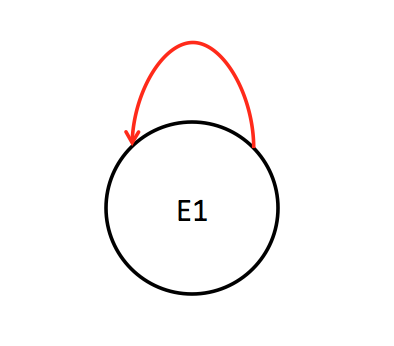
\includegraphics[scale=0.5]{selffeedback}
	\caption{\it Simple feedback loop with an entity supplying its input from its output.}
	\label{fig:exampleselffeedback}
\end{figure} 
Feedback loops can be encompass multiple entities, in Fig.~\ref{fig:exampletwofeedback} a feedback loop is shown that encloses two different entities. A output from $E2$ is passed to $E3$ which in turn creates a new input for $E2$, though $E2$ input is not directly its own output, it does depend upon it. 
\begin{figure}[H]
	\centering
	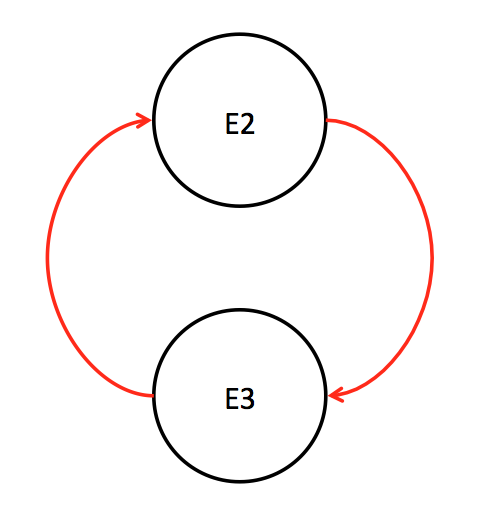
\includegraphics[scale=0.5]{twofeedback}
	\caption{\it Feedback loop between two entities, with each output being transformed by the other entity before becoming an input.}
	\label{fig:exampletwofeedback}
\end{figure} 
A loop such as the one in Fig.~\ref{fig:exampletwofeedback}, is only considered a feedback loop if information is passed through out the entire loop. If $E3$ produced a constant output, or an output that does not depend upon its input from $E2$, then this would not be a feedback loop as the new input to $E2$ does not depend on its output.

These example are very simple, feedback loops can be much more complex, encompassing any number of entities, each of whom can have very complex algorithms for transforming their inputs. Feedback loops can operate across time, meaning that an event in the past can eventually feedback to a present decision. For a feedback loop containing a large number of entities the time scale on which the feedback occurs can be come significantly large.

Though feedback loops are often assumed to be a negative property, some can be stabilising due to a benign effect.

Feedback loops can be present in a system in two ways, either they can be a constant fixture, called a static feedback loop, or they can form and change, called a dynamic feedback loop. A static feedback loop is present in the system from the start whether this is intentional and known, or unintentional and unknown to the members of the system. Dynamic feedback loops may not be present at the start and can form and change over time, with new entities joining or leaving them, allowing them to increase or decrease in size or effect, to split or merge, or to disappear.

Due to the potential complexity of feedback loops both in construction and in time, they can be difficult to detect, therefore methods are usually used to expose them. For static loops, forms of static analysis can be used such as, analysing initial setup, this is possible since the loops do not change through out time. Dynamic loops can be much harder to observe and analyses, an important aspect to detecting these loops is the interactions, messages sent between different entities within the system. Since the loops can evolve over time being able to track and analyse these messages over a time series is vitally important for the analysis of these loops, this time dependent analyse is called dynamic analyse.

Since feedback loops can be destabilising and damaging to the system in which they occur, there is interest in studying this emergence in the aim to prevent monetary loss and damage to the economy.

A notable form of emergence behaviour, due to feedback loops, that takes place within the electronic markets are flash crashes. A flash crash is an event during which time the trading price of a security drops very rapidly, becoming disconnected from its fundamental, before then recovering~\cite{rareeventflashcrash}. A particularly famous flash crash is that of 2010, in which the E-min S\&P 500 equity futures market dropped in price by more then 5\%, before rebound to close to its original price~\cite{SECreport_delays, rareeventflashcrash}. This whole process occurred very rapidly, lasting approximately thirty-six minutes and has been described as``one of the most turbulent periods in their history'' for the US financial markets~\cite{Impact_hft}.

Research done by Ref~\cite{DynamicCoupling_Chris, otherabmflash}, describes how the crash may have unfolded due to a feedback loop between High-Frequency Traders (HFTs), known as `hot-potato'' trading.

HFTs are a subset of algorithmic traders who normally participate in the market as arbitrageurs or market makers, they invest in ultra-high speed technology allowing them to detect, analyses and react to market condition in nanoseconds \cite{hftinformation1}. This means HFTs can trade huge quantities of assets in very short time frames, with some estimates stating that 10-40\% of all trades where initiated by them during 2016 \cite{hftmarketparticipation}.

The feedback loop of ``Hot Potato'' trading, is when inventory imbalance is repeatedly passed between HFTs market makers. A market maker is a trader who is required to have both a bid and a ask on the order book at all times, this means in theory that they are constantly buying and selling, a high frequency market maker as expected should be buying and selling very very often. Market makers make a profit from the spread and not long positions, hence they want to keep inventories low to avoid the market moving against them. To achieve this market makers have strict inventory limits that if they pass will cause them to go into what is know as a ``panic state'', during this state the trader will sell of an amount of its inventory to return back into its normal trading region. This inventory now sold by the market maker can be bought by another market maker causing them to in turn go into ``panic'' and sell, this process is ``Hot Potato'' trading and can in theory continue indefinitely~\cite{Elias_Paper}.

This constant selling and buying of inventory can artificially inflate the trading volume of the market, changing how many traders operate and potentially leading to a flash crash.

Flash crashes have occurred on a number of occasions and in a large selection of markets, with a more recent example being a crash of the cryptocurrency ethereum~\cite{cryptocrash}.


%%%%%%%%%%%%%%%%%%%%%%%%%%%%%%%%%%%%%%%%%%%%%%%%%%%%%%%%%
\subsection{Methods for Modelling Emergent Behaviour in Finance}  \label{litreviewofabmrr} 
There are many different methods available for modelling system that may exhibit emergent behaviour, such as: 1-period, 2-period and multi-period models, probabilist models, like hidden Markov models, ordinary differential equations and partial differential equations [REFS??????]. This paper focusses on two models that can be used for discrete non-equilibrium system, recurrence relations and agent-based models. 

Both recurrence relations and agent-based models have been used in modelling the financial markets and have had a number of papers published on them.

Recurrence relations have seen wide spread use in economics appearing in a large selection of journals, including numerous times in top journals~\cite{rra10, rra1, rra2, rra3, rra4, rra5, rra6, rra7, rra8, rra9}. This wide spread use of the technique implies the acceptance of recurrence relations within financial modelling.      

Agent-based models also have a large selection of papers published on them relating to economics and finance~\cite{ abma2, abma3, abma4}. However these papers are noticeably absent from top economics journals (with some exceptions, such as Ref.\cite{abmexp1} and~\cite{abmexp2}) and tend to be published in the Journal of Economic Behavior \& Organization and the Journal of Economic Development \& Control~\cite{whereabmp, farmerfoleynature}. The lack of agent-based models present in top economic journals combined with the number of papers published in other journals shows the lack of wide spread acceptance for this technique~\cite{agbntj, econmistsnoabm, lob_noecomimists}.

Here these two modelling techniques will be described.  


\subsubsection{Recurrences Relations} 
Recurrence relations connect a discrete set of elements in a sequence, these elements are normally either numbers or functions, they can be used to define these sequences or produce the elements in them. They can be seen as equations that give the next term in a sequence based on the previous term or terms, hence defining said sequence. Recurrence relations are often used to define coefficients in series expansions, moments of weight functions, and members of families of special functions~\cite{recurrelationbook}.

The most simplistic form of a recurrence relation is one where the next term depends only on the immediately preceding term. If the $n^{th}$ element in the sequence is defined as  $x_{n}$, then this recurrence relation can be written as,    
\begin{equation}
x_{n+1} = f(x_{n}),
\end{equation}
where $f()$ is a function that calculates the next term based on the previous one. A recurrence relation does not just have to depend on its immediate previous term and can depend on any number of terms further back in the sequences, for example a recurrence relation depending on terms from two and three steps before can be written as, 
\begin{equation}
x_{n+1} = f(x_{n-1}, x_{n-2}),
\end{equation}
with $f()$ now taking two inputs to produce the new term in the sequence~\cite{recurrealtionwebpage}.

Recurrence relations can also be used to define a sequence through time, in the simplest case the enumerate $n$, can be set to represent time $t$, this is applicable to discrete time as it requires set steps between the different times. Just as in the previous examples, the simplest recurrence relation is,  
\begin{equation}
x_{t+1} = f(x_{t}),
\end{equation}
where $x_{t}$ is the term at time $t$ and $f()$ gives the term at $t+1$ based on the term at $t$. Again this can be expanded to include terms from a number of previous time steps, allowing the memory of the sequence to be shown.
 
A recurrences relation for defining a sequences may as well as depending upon previous terms, also depend upon some parameter, $\alpha$, this would give, in its simplest case, 
\begin{equation}
x_{n+1} = f(x_{n}; \alpha).
\end{equation}
The next term in the sequence may not only depend on previous terms within its own sequence and parameters, it can also be conditional on another sequence. For example one sequence through out time, $x$, may depend on another sequence through out time, $y$, a simple recurrence relation for this could be,
\begin{equation}
x_{t+1} = f(x_{t}, y_{t}),
\end{equation}
with the sequence for $y$ possibly depending on its own recurrence relation. The sequence for $x$ may not even directly depend on its own sequence and could solely depend on $y$, 
\begin{equation}
x_{t+1} = f(y_{t}).
\end{equation}
Though it could also indirectly depend on its self, if $y$ was defined by a recurrence relation depending on $x$, such as, 
\begin{equation}
y_{t+1} = f(x_{t}).
\end{equation}
These cross sequence associations allow for complex interactions to be represented as time series defined by recurrence relations.

Recurrence relations have a number of benefits given by their construction, such as:
\begin{itemize}
    \item Giving a formal mathematical definition of the whole system.
    \item Showing an obvious link between equations within the system.
    \item Giving a static representation of the system.
\end{itemize}

A formal mathematic definition of the whole system being model is given when using recurrence relations due to three factors: the way in which they model the whole system as a entity, the static view point they give to the system and the mathematical stye which they take~\cite{rrformulism}.  %is this right?

Links within sets of recurrence relations are hard coded into the equations, making these relationships amenable to static analysis.      

This model lays out both the functionality of each equation and the relation between them in such a way to give a static representation of the system as a whole. 

This model however has difficulties in design as it can be challenging in creating a large continuous description of a system containing many components, also the function calls as a method of information passing can make dynamically tracking the flow of information during a simulation hard [REFS????].   




%These cross sequence associations allow for complex interactions to be represented as time series defined by recurrence relations, this is a method which can be applied to agent-based modelling.

%Reference~\cite{econmistsnoabm} showed how an agent-based model looking at the microstructure of the financial markets, can be exhibited in the form of recurrence relations. In their approach each agent with in an $n$ agent model is considered to be well described by a state variable, $x_{i, t}$. The state variable describes the agent at each time step, where $i$ is the identity of the agent $(i \in 1,2,....,n)$, and $t$ is the time step at which the agent is being described, i.e. $x_{1,5}$ describes the first agent at the fifth time step. These state variables are defined by the recurrence relation,     
%\begin{equation} \label{eq:notimedelayrecur}
%x_{i, t+1} = f_{i}(x_{i, t}, x_{-i,t}; \alpha_{i}),
%\end{equation}
%where $f_{i}()$ is a function unique to agent $i$, that can take the state of the agent at the previous time step, $x_{i, t}$, the state of any other agent at the previous time step, $x_{-i, t}$\footnote{The $-i$ is used to refer to all other agents in the system. So if $i=1$, $-i$ refers to agents $2,3,4,....,n$, for an $n$ agent system.}, and a bespoke parameter $\alpha_{i}$.

%This method works by describing each agent as a sequence of state variables, these sequences are then interlinked by having dependencies to each other, allowing both the agents and their interactions to be represented. A simple example of this could be two agents, $x_{1}$ and $x_{2}$, that are coupled to each other and only depend on the others value at the previous time step and a parameter, represented by the recurrence relations,     
%\begin{equation}
%x_{1, t+1} = f_{1}(x_{2,t}; \alpha_{1}),
%\end{equation}
%\begin{equation}
%x_{2, t+1} = f_{2}(x_{1,t}; \alpha_{2}).
%\end{equation}
%This formulation only shows relationships to the previous time steps, however information delays can be added to the system by allowing the recurrence relations to have a longer memory. A recurrence relation that uses a state variable from three time steps ago, could be considered to have a time delay of three time steps in receiving this information. The generalisation of the model needed to allow for this, is a recurrence relation of the form, 
%\begin{equation}
%x_{i, t+1} = f_{i}(x_{i, t}, x_{i, -t} x_{-i,t}, x_{-i, -t}; \alpha_{i}).
%\end{equation}
%This is similar to Eq.~\ref{eq:notimedelayrecur} but contains two new terms $x_{i, -t}$ and $x_{-i, -t}$, these terms are used to refer to any time steps before the previous one, time $t$. This more general equation can now reference any state variable from any previous time, from any agent, as well as its bespoke parameter, to compute the next term in its sequence.
 
%This models can be solved for macro-level properties by iteratively solving each state variable, $x_{i, t}$, given some initial conditions. This method of assessing the model gives it a formal definition, and one that is accessible by a larger range of experts then classic agent-based models. Recurrence relations in a number of forms are commonly used in economics and finance and hence are familiar and relatable to economists, this makes them a far more effective tool for describing models to these domain experts then agent-based models.

%This iterative method for solving the equations makes any dependencies between systems apparent, as if $x_{2, t}$ is present in the definition of $x_{1, t+1}$, one can say that $x_{1,t+1}$ depends on $x_{2,t}$. This transparency of dependencies makes this formulation amenable to static analysis, allowing the recurrence relations to be investigated to return their static dependencies.

%Although all recurrence relations will contain some form of recursive, since this is an intrinsic property, this will not necessarily be negative or destabiliszing. For example a dependency on a state at a previous time step may not be destabilising to the system, however the reverse would be a case where the state variable at $t+1$ depended on its self, this would be a destabilising loop. Static analysis hence could be used to detect hard-wired destabilising loops, such as the one just mentioned.

%Static analyse of the system can become difficult when the functions $f_{i}()$ contain conditional statements relating to their inputs, this can cause inputs not to be used at certain times hence meaning dependencies will not be as obvious as simply the inputs given, this is a problem of determining wether a function will necessarily evaluate all its arguments~\cite{willevaluteargsa}.

%Though through static analysis recurrence relations can be used to view the history of the state variables of a single agent, however the history of messages between pairs of agents is not easily detectable with static analysis. The interaction history is found through dynamic analysis which is not well suited to recurrence relations, as they lack a clear ability to follow the passing of messages within the system.   








\subsubsection{Agent-Based Models}
A modelling technique that takes a more dynamic approach is agent-based modelling. Agent-based modelling can be considered more of a mind set then a rigid methodology, this involves describing the system in question in terms of its components and then allowing these to interact. Agent-based models allow a system to be described naturally and are hence the canonical approach to modelling emergent phenomena. This method is a bottom up approach, allowing for each component of the system, agent of the model, to be created to a relevant degree of abstraction~\cite{abmhumsystems}.

Agent-based models have been used to model a wide range of emergent behaviour including in the financial markets, examples of this are, noise traders~\cite{abmnoisetraders}, herding among traders~\cite{abmherding}, and fundamentalists~\cite{abmfundemetilists}.

Agent-based models are particularly suited to system which, contain a number of autonomous components. Each component can be modelled independently and then allowed to interact through messages sent between each other. This allows for a obvious visual design of the system, such as that shown in Fig.~\ref{fig:abmii}.
\begin{figure}[H]
	\centering
	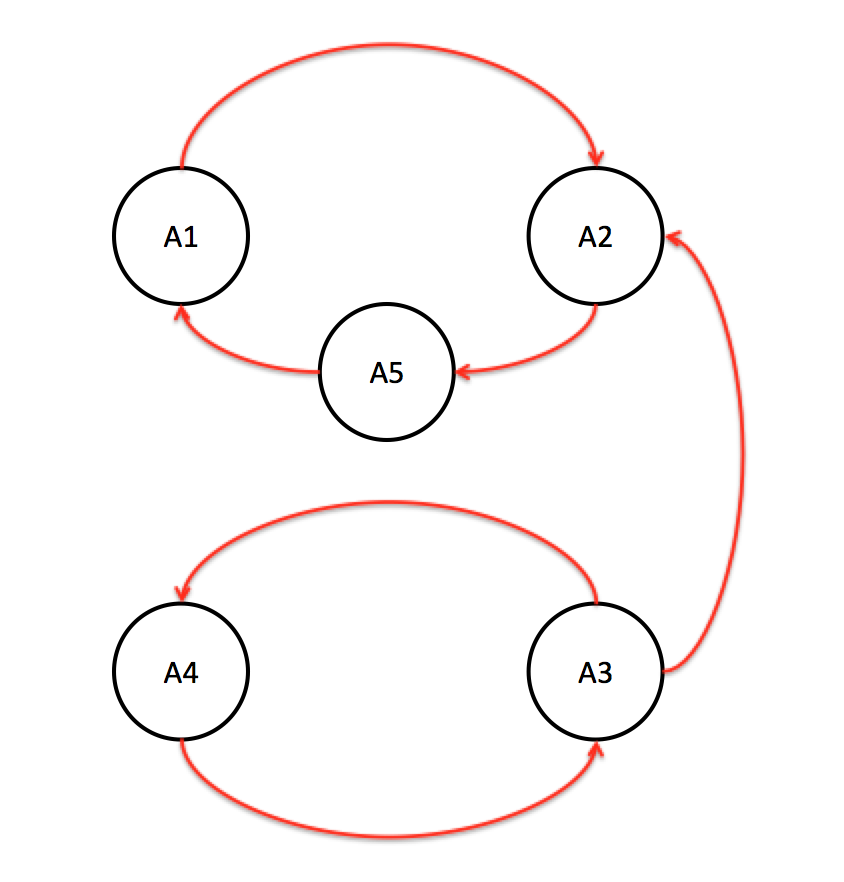
\includegraphics[scale=0.5]{abmii}
	\caption{\it Visualisation of the allowed interactions between five different agents, represented by black circles, with red lines representing the message paths.}
	\label{fig:abmii}
\end{figure} 
The main aspect of this model is the agents used. Though every system modelled can have drastically different agents, there are a few characteristics which should be in place for a agent to be considered an agent~\cite{MN2010, abmtsd}:
\begin{itemize}
   \item An agent is self contained, unique and identifiable, this requires an agent to have boundaries which can easily be used to determine what is and what is not part of the agent. 
   \item An agent autonomous and it can act independently during its interactions with other agents. Its has behaviour and decisions that can be associated with information acquired  during communication with other agents. 
   \item An agents state varies over time, representing variables associated with its current position. 
   \item An agent behaviour is influenced by dynamic interactions with other agents. 
\end{itemize}

This modelling technique has a number of benefits originating from its construction, these include:
\begin{itemize}
   \item Being able to independently create each agent to varying degrees of complexity. 
   \item Giving a clear visual representation of the systems interconnectedness.
   \item Giving a dynamic representation of the system.
   \item Easily expandable by adding more agents.  
\end{itemize} 

Since each agent in the system can be completely autonomous and independent from each other, save for message passing, this allows for them to be created individually. Hence each agent can describe its relevant component to a relevant degree of complexity, making the creation of a simulation more intuitive and sectioned. This makes agent-based models in many cases the most natural way for describing systems composed of ``behavioural'' entities~\cite{techsadsProbsabm}.

Do due the set up of this model the a network representing the communication between different agents is easy to construct, this allows for topologies to be visualised and can aid in the creation of a simulation.    

The use of messages and bottom up approach this model takes allows for a more dynamic view of a system to be achieved, messages can be more easily tracked through out the systems evolution allowing for events to be more easily pinpointed and analysed.  

The use of independent agents makes this technique very amenable to expansion, new agents can be added normally with little to no change to previously existing agents. This allows these simulations to be confidently expanded to look at more complex systems, or to add new elements to an existing system.  

These aspects of this approach make the modelling technique well qualified for modelling and analyse of emergent behaviour within systems of interacting components. However this approach does contain some draw backs including a one-to-many problem (where though some high level behaviour may be noted in the system this does not mean the only way of achieving this behaviour is the current system design) and the lack of a formal definition for the system as a whole [REFS???].  



%%%%%%%%%%%%%%%%%%%%%%%%%%%%%%%%%%%%%%%%%%%%%%%%%%%%%%%%%
\subsection{InterDyne} \label{InterDyne_section}
An example of an agent-based model used in modelling the financial markets is InterDyne. InterDyne is bespoke simulator created by Clack and his research team at UCL~\cite{Chris_webPage}, it is a general-purpose simulator for exploring emergent behaviour and interaction dynamics within complex non-equilibrium systems.

InterDyne design is that of an agent-based model interacting via a harness. This creates a structure of individual autonomous agents who interact through messages sent through a harness to one another.
 
Similar to other agent-based models InterDyne operates in discrete-time rather then continuous time. These quantised time chunks, which move the simulation forward, can be left without proper definition (allowing operations to be defined in a number of time steps) or they can be equated to a real time (usually with the smallest time gap needed being a single time step and then all other timings being integer multiples of this). This discrete time is most important to message passing, with messages between agents are only sent on a integer time step.

Massages in InterDyne are just small packets of data, such as a series of numbers. An agent can send private messages that are only received by a single other agent (one-to-one messages), or it can send public broadcast messages received by any number of other agents, subscribed to a channel (one-to-many messages). To facilitate this a communication topology can be made for InterDyne, this is done in the form of a directed graph determining which agents can communicate with each other. Due to the directional nature of these messages this topology could allow an agent to send messages to another but not be able to receive messages from that same agent. Messages have a defined order to them, an agent will, unless otherwise instructed, always process messages in the order in which they arrive. To change the order in which messages arrive delays can be added to communication paths between agents, this can be a static delay which always applies to messages sent from one agent to another, meaning this will arrive a set number of time steps later. Or a more complex dynamic delay, which is achieved by using another agent to mediate the passing of these messages delaying by an amount decided on in some internal logic. All messages in InterDyne are passed through a harness, this does not alter the messages or delay them\footnote{Unless instructed to, using a static delay.}, but does store the messages and their order which can be used in post analyse.
        
Each of the agents within an InterDyne simulation can be completely unique and modelled to different levels of complexity, as is the case with most agent-based models. As a whole InterDyne simulations are deterministic, repeated experiments will return identical results. However non-determinism can be added via the agents, making some part of an agent stochastic will lead to repeated experiments on the whole returning different results. A pseudo-random element can also be added by instructing InterDyne to randomly sort the message order for any agent receiving multiple messages in one time step. This is only pseudo-random as, as long as the same seed is used each run of the simulation will order the rearranged messages in the same way.\footnote{If an agent receives multiple messages at the same time step and the pseudo-random element is not being used, these messages will order based on the identifiers of their sender agents.}

InterDyne is created to be particularly amenable to dynamic analyses of its simulations, this is achieved in part by all messages being sent via the harness allowing them to be stored in order.     


\subsubsection{Applicability to Finance} \label{applicabilut_to_finance}
InterDyne has been designed with modelling flash crashes in the financial markets in mind and has a number of features that make it well suited to this purpose. 

\paragraph{Deterministic}
The deterministic nature of InterDyne allows for experiments to be run multiple times with the same result always returned, this allows for changes to the experiment setup to be investigated. For example changing the number of traders in the market and comparing this to a previous run allows for an investigation into how many traders are required for emergent behaviour to be observed.

This becomes particularly interesting when comparing the interactions between market makers to that of the n-body problem. Like with this problem one could expect emergent behaviour might occur to some extent in a large group of market makers, however the question of whether emergence persists in a comparable market to the three-body problem and how this compares to a larger market can be investigated.   

\paragraph{Message Delays}
Allowing for messages to be delayed is needed to facilitate hypotheses involving delays as a factor for emergent behaviour. Delays have been suggested to have caused ``hot potato'' trading during a flash crash, these delays can exist due to processing time and transmission time of messages~\cite{SECreport_delays}.

InterDyne allows for both symmetric and asymmetric, delays. These delays can be static or dynamic, with dynamic delays requiring a special intermediary agent. 

\paragraph{Storing Messages}
InterDyne facilitates analyses of simulations be allowing for the messages between agents to be stored and viewed as a trace. This can include all messages as well as timings, messages can also be sent directly to the harness which will be added to the trace file. 
  
\paragraph{Message Ordering}
The order in which messages are processed can be very important. For example in an exchange, it can change whose limit order has priority at a given price and whose market order executes the lowest prices. Changing these factors can make or break feedback loops within the system, meaning if message ordering is not properly dealt with the correct emergent behaviour may not be observed. Hence InterDyne stores messages in the order they are received by an agent, taking into account delays to the messages. This however can not be done when multiple messages are received at the same time step, due to the nature of discrete time there is no way for the agents to know which message arrived first. Therefore two options are presented by InterDyne; messages are ordered according to their agent identifier or messages are randomised and executed in the emerging order.



\subsubsection{InterDyne Detailed Operation}
InterDyne is a written in the functional language Haskell. The structure of an InterDyne model is show in Fig.~\ref{fig:harness_setupfigure}, this structure contains a number of agents and a simulator harness. These agents send two types of messages, either one-to-one or one-to-many (broadcast) messages. Both these messages are sent to the harness, the harness then resends these messages to the appropriate agents, one-to-one messages are sent to their target agent and one-to-many messages are sent to any agent subscribed to the relevant broadcast channel. Messages can also be sent directly to the harness and not rerouted to another agent. At the end of the simulation the harness will produce a trace file containing information on all the messages sent for post-hoc analysis.    
\begin{figure}[H]
	\centering
	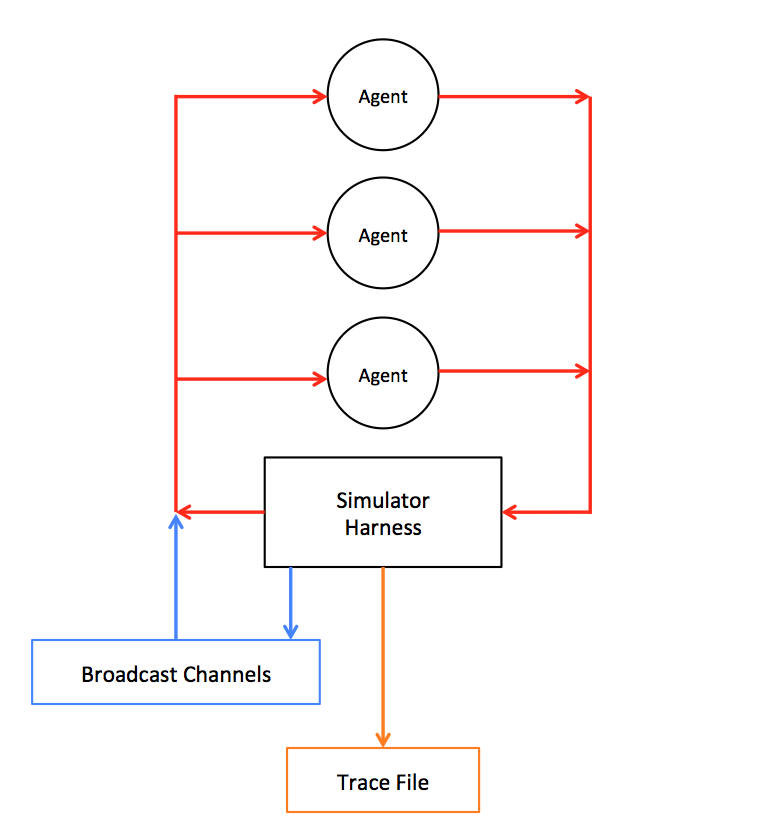
\includegraphics[scale=0.5]{harness_setup}
	\caption{\it Structure of an InterDyne simulation containing three agents. The messages sent by the agents to the harness and from the harness are coloured red. The trace file and messages sent to the trace file are coloured orange. The messages sent from the harness to the broadcast channels and then back to the agents are coloured blue~\cite{interdynemanual}.}
	\label{fig:harness_setupfigure}
\end{figure} 
%-topology and delays 
InterDyne has a intrinsic delay, which means any message sent will not be received until the next time step, message sent at $t$ will be received the earliest at $t+1$. This is in part due to the fact that the harness compiles all messages from a single time step before sending them to their targets and hence initiating the next time step. The harness can be seen as the driver in the simulation sending out the message and forcing the agents to send there next message.   

Longer delays can also be added using InterDynes topology, this allows for any two agents to be selected (a sender and a receiver) and for a delay between them to be given. This topology takes the form of a directed graph, with the agents acting as the nodes and the interaction routes as the links, this allows for the delays to be asymmetrical. Using this a delay for a path could also be set as a abort message, making a particular communication route unusable.  

Adding delays is done through run time arguments, here two run time arguments must be added, one stating the maximum delay in the system and the other listing the delays. To show the maximum delay the argument $(Arg (Str$  $``maxDelay", 10)))$ is used, where $10$ is the maximum delay. To add the list of delays the argument $(DelayArg (Str$  $``DelayArg", delay))$ is used, where $delay$ is a function that takes two agents and returns the delay between the first and the second. 
%-what a message looks like 

Messages sent between agents can in theory be as complex as needed, these messages do however have to comprise of these components: 
\begin{itemize}
   \item A tag indicating the type of message being sent, e.g. a broadcast message.
   \item A tuple of two integers, with the first being the sending agents ID and the second being either the receiving agents ID or the receiving broadcast channels ID.  
   \item The data that is being sent. 
\end{itemize}
An example of this is a one-to-one message, which would look like $Message$ $(1, 2)$ $data$, where $data$ is the information being sent from agent $1$ to agent $2$ 

A broadcast message, which looks like $Broadcastmessage$ $(3, 1)$ $broadcastdata$, can be received by agents subscribed to its channel, in this case $1$. All agent subscriptions have to be announced at the beginning of a simulation and can not be changed during it. This is done by adding the subscription channel to the list in a tuple passed as an argument, for example this could look like $(agent1, [1])$, for agent 1 subscribed to broadcast channel one.

Empty messages can also be sent, if the message is required to be known to be intentionally empty and not a mistake the a message can be sent containing ``Hiaton''. This is done at the beginning of the run to allow for the harness to send a first message. 
%-what is an agent in interdyne and what is its type

InterDyne is designed in such a way that agents both taken in and produce a seemingly infinite list of messages. This is achieved through lazy evaluation in Haskell, which in short means that any element in the list will not be calculated until it is absolutely needed. This allows for an infinite list as long as no agent tries to read further into the list then what as already been calculated. In achieving this an agent must at each time step, allows read in a message (even if it is then not used) and produce a list of messages (even if this is a empty list). An agent will hence iterate over the list of incoming messages, at each time step adding a new output message to its list of output messages.  

Agents in InterDyne are topically, though not required to be, written in two parts, a wrapper function and a logic function. The wrapper will manage the reading of inbound messages to the agent and generate its outbound messages, it will also update the local state of the agent. While a logic function is called by the wrapper to calculate the messages to be sent and there content. A agent written following this design could have a form similar to that of the agent show in Fig.~\ref{fig:wrapperfrominterdyne}. This agents wrapper recursively calls its self on the inbound message list, consuming the head of the list\footnote{This design dictates that the head of the list is the messages for the current time step.} and producing a list of outbound messages using a logic function.  
\begin{figure}[H]
	\centering
        \lstinputlisting[language=Haskell]{complexagentwrapper.hs}
	\caption{\it Simple wrapper function, which creates a list of output messages by iterating through a list of inbound messages and calling the sub-function $logic$.}
	\label{fig:wrapperfrominterdyne}
\end{figure} 
%-what is the harness in interdyne and what is its type

The simulator harness is an intrinsic part of the simulator, it drives the simulation, handles message passing and produces the output trace file. %need to put more here, whats its type, what does it look like?

%dont say paper 
%The simulator harness is embodied in the function called sim, the actual function sim in interdyne contains not only code to run the simulation but also code associated with writing to trace files and other admistrative funtions. for the purpioses of this project, we use the following reduced sprecification of the fucntion sim which captures the all of the core fuctionality for managing message passing for agents and driving evaluation of the simualtion

%-how do you run an interdyne experiment 

Running an InterDyne experiment is done by calling the simulator with relevant inputs, an example example of this is shown in Fig.~\ref{fig:runninginterdyne}.
\begin{figure}[H]
	\centering
        \lstinputlisting[language=Haskell]{interdynewithdelays.hs}
	\caption{\it A run of an experiment in InterDyne containing delays.}
	\label{fig:runninginterdyne}
\end{figure} 









%%%%%%%%%%%%%%%%%%%%%%%%%%%%%%%%%%%%%%%%%%%%%%%%%%%%%%%%%%%%%%%%%%%%%%%%%%%%%%%%%%%%%%%%%%%%%%%%%%%%%%%%%%%%%%%%%%
\section {Description and Analysis of the Problem} \label{despriptionandanalysproblem}

Investigating emergent behaviour originating from interaction dynamics, within a complex system, relays on viewing the communication between different components of the system as messages being passed. These messages can then be analysed to assess the communication and its pattern that lead to the creation of the emergent behaviour, this approach is amenable to the discovery of phenomena, such as dynamic feedback loops. A model investigating emergent behaviour hence must be able to view communication as messages being passed between different components. For results from this model to be broadly accepted, in fields such as economics, the model as a whole must also be well defined.      

Agent-based models naturally support a message passing view making them well suited to analysing and investigating emergent behaviour. However most agent-based models, though having each individual agent be fully specified, do not have a well defined formalisation for the system as a whole. This makes it challenging to perform system wide analytics on most agent-based model. Recurrence relations naturally support a system wide analysis, due to the full definition of their models. However their formulation does not support a message passing view of communication between components, making it difficult to analyse emergent behaviour with them directly. 

This creates a problem as neither model is perfect for the task at hand. A resolution to this problem suggested by Ref.~\cite{econmistsnoabm}, is to give a formal definition of the specification of an agent-based model as a set of recurrence relations.This can be seen as viewing a system in two ways, as a recurrence relation model and as a agent-based model, a two-views approach.

This section how a two-views approach can be created and problems associated with the design of this method. 

\subsection{Method for Achieving a Two-Views Approach}
%%%%%%How can this solution be achieved (translation form rr to abm)
A two-views approach, where recurrence relations define the formalisation of an agent-based model, must consist of a connection between the two models. This connection must be able to show that the recurrence relations and the agent-based model represent each other.  

%we know a translation is possible as all abm can be written in a rr form
%Epstein (2007) invalidates the commonly cited dichotomy between computational agent-based models and equation-based models by proving, albeit informally, that all computational agent-based models can be expressed using partial recursive functions. Epstein begins his proof by observing that because any standard computer program is effectively Turing complete, then programs for computational agent-based models must be so as well. Epstein then notes that there is an equivalent partial recursive function for every Turing machine. Therefore, there are sets of partial recursive functions for every computational agent-based model. These partial recursive functions are equations that fully specify any given computational agent-based model. Epstein also uses the partial recursive functions approach to argue informally that computational agent-based models, particularly those in the social sciences, are deductive in nature.

%%%%%%what is a translation between rr and abm
A translation between between a set of recurrence relations representing a system to an agent-based model representing the same system. This will give a connection between the two models which is able to demonstrate the equivalence of the recurrence relations and the agent-based model, hence allowing for the former to act as the formalism for the latter.   

%%%%%%what direction should this translation take and why? rr -> abm
An important consideration in creating a translation between the two methods is, which direction this translation should take. For the purpose of defining the formalisation of an agent-based model and hence increasing its acceptance for a reader, a recurrence relations to agent-based model trajectory is preferred. This ordering will allow a read to start with a formalised description and translate this formalisation to cover an agent-based model, as opposed to starting with an unformalised model and translating to a formalised one.     

%%%%%%How will this translation be done? look at work other people have done on translations (step-by-step) 
The next consideration is how this translation will be achieved. Inspiration can be drawn from other works investigating the design of translations, such as Refs.~\cite{clovertrans},  \cite{transproggotmod} and  \cite{stepcorentconv}. These three papers discuss translations between program representations in a way in which, the final representation will faithfully represent the initial. The approach taken by these papers is to increment the translation in step-by-step manner, where each step slightly transforms the previous to be closer to the final form. The benefit of this method is that if each step on the translation can be proven to be correct then the whole translation can be seen as correct. 

%%%%%%what is the project? (make rr language, convert in a step-by-step manner to InterDyne)
A two-views approach can hence be created by translating in a step-by-step fashion from a recurrence relation language to an agent-based model. The agent-based model used in this translation is InterDyne and the recurrence relation language used is discussed in Section~\ref{beskoperecurrancerealtion}. InterDyne was selected due to a number of factors, most importantly InterDyne was designed from the bottom up to model and investigate emergent behaviour with the financial markets, with research already being conducted using it to this end~\cite{DynamicCoupling_Chris}, this software was also a convenient choice due to access to the source code and local expertise.

\subsection{Review of Similar Work}\label{simwork}
The idea of using recurrence relations to give a formal definition to an agent-based model is not a novel one and falls under the general heading of using formal systems to prove properties of agent-based models. Work in this area has covered formal using game theory, discrete systems, classifier agents and equation-based models~\cite{taabm}. The use of recurrence relations falls under the classification of an equation-based model, these have been used in a number of papers looking to give a formalisation to agent-based models. Here three papers, Refs~\cite{ebmabmi}, \cite{econmistsnoabm} and \cite{abmtsd}, looking at this area will be reviewed and discussed, along with DEVS formalism introduced in Ref.~\cite{introdevs}.

Before reviewing these papers, it is worth considering the more obvious question of does a formalism need to be given by another modelling technique to allow for the analyses of an agent-based model? Reference~\cite{taabm} present a method formalism for the analysis of agent-based models, looking in particular at performance. 

This paper looks to prove findings from agent-based models, in particular the focus is on existing agent-based software such as Swarm, Repast 3 and others. This paper notes that these pieces of software use a modular imperative architecture with factored agents, spaces, a scheduler, logs, and an interface. Hence this paper presents a theoretical formalism for analysing a modular imperative agent-based model.    

This this formalism is presented using an abstract machine specification of the modular imperative agent-based modelling architecture. A  Random Access Stored-Program (RASP) architecture was chosen for the abstract machine, this architecture had been created in an earlier paper (Ref.~\cite{raspceated}) and was chosen due to its similarities to real computer systems. This is opposed to other options including Turing machines and $\lambda$-calculus, as they are less well matched with real computer systems.     

One of this papers motivations for using this technique over an equation-based model formalisation, is that the authors feel that this formulation of the agent-based model in terms of an equation-based model would be unnatural and possibly unrecognisable to those accustomed to agent-based models. This consideration is not as important to the work presented in this dissertation, since here the aim is to familiarise those accustomed with equation-based models to agent-based models and not the reverse. The same argument applies to the use of RASP over alternatives such as $\lambda$-calculus, this dissertation is more interested in creating a formalism which is relatable to economist over computer scientists.   

The first paper to be examined is Ref.~\cite{ebmabmi}, this paper considers the formalisation of agent-based models by creating their implementation guided by equation-based models, an (equation-based model)-oriented design.  

This paper looks at an example with interacting entities with given strategies, however these strategies could change upon interactions. In this example the equation-based model took a probabilist and macro-view approach where the agent-based model, due to its nature, to a micro-view approach. The analyses of these two models showed that though the systems appeared to be the same the micro-view approach could create slightly different outcomes depending on the number of agents chosen. This difference comes from the fact that the individual agents in the agent-based model were created to match a macro-level description given by the equation-based model, however due to the autonomous nature of the agents only their general behaviour can match and in certain circumstances even this did not correctly produce the behaviour.

This paper concludes summarising the benefits of this approach in validating an agent-based model, here an agent-based model is known to be a faithful representation of the system as long as the equation-based model is a faithful representation. However the question of whether the age-based model is correctly implemented still rests with that model. 

The main difficulties faced by this paper appear to be the transformation from a macro-level view (equation-based model) to a micro-level (agent-based model) view, this is particularly apart due to the statistical nature of the equation-based model. Though they succeeded in creating a formalisation of their model the differences in results between runs still raises questions over the equality between the two view points. To avoid this issue, taking a more micro-level focussed equation-based model should suffice.

The next paper is Ref.~\cite{econmistsnoabm}, this paper is based on a similar principle to this project in that it seeks to bridge the conceptual gap around  agent-based models in economics. It tackles this problem by introducing an equation-based formalism to describe both agent-based models and analytical models, though of interest here is their work on former. 

The agent-based model is formalised by specifying how each agent\textsc{\char13}s state within the model changes between each time step. This is done by defining agent attributes using vectors of state variables and then applying time-indexed difference equations to specify each agents state change. This allows for expression of the agent-based model in terms of difference equations, which they then use to look at parameter estimation. 

Their work shows the ability to prefer estimations on agent-based models, counter to some criticism that has been levelled at agent-based models. Some difficulty in this approach can come from agent-based models with complicated algorithmic behaviour within the agents, specifying these models as difference equations can be challenging task. The work in this paper does not directly suffer from this problem as all systems are first described as recurrence relations before being translated into agent-based models, meaning that the equation view will only be as complex as the original writer intends.  

Th last paper to be looked at is Ref.~\cite{abmtsd}, this paper investigates relating Forrester\textsc{\char13}s System Dynamics (SD) model to an agent-based model. System dynamics models consist of a set of difference equations, so this can be seen as a comparison between difference equations and agent-based models. This paper presents a formal specifications for both the Forrester\textsc{\char13}s and agent-based models, these specifications are then compared to show their equivalence. Was equivalence has been proven the specification of a Forrester\textsc{\char13}s model can be used to derive an agent-based model that is an correct representation of the same system.

This technique its applied to an SIR epidemic model, creating an Forrester\textsc{\char13}s and agent-based model representation. These two descriptions of the system are then evaluated and have their results compared. The findings show that though both models show similar behaviour, there is not an exact match between them. This is due to the probabilistic nature of the system being modelled and the different approach that an agent-based model takes to these kind of systems. 

This paper, though showing equivalence, does so in a more abstract manner then a direct translation between the two models. The difference in experimental results from the two models is down to the use of describing the system in a probabilist fashion, this can be avoided by describing a system in a more micro-level view.    

A discussion relating to the formalism of agent-based models would be amiss with out mentioning the Discrete Event System Specification (DEVS)~\cite{introdevs}. DEVS is a theoretical formalism designed for analysing complicated simulations, which it does by describing simulations as hierarchical Moore machines, with additional timing information added to the state transitions. DEVS has a few variants including classic DEVS (this is the core abstraction), coupled DEVS (allows for hierarchical nesting of the Moore machines~\cite{coupleddevs}) and Dynamic Structuring DEVS (attempts to allow for dynamic behaviour~\cite{dynamicdevs}).

DEVS is able to provide a theoretical foundation for analyses of a number of critical computational properties of agent-based models, including properties such as decidability. In theory DEVS has the ability to represent any computational model, including agent-based models, as following the Church-Turing thesis any computing system as complex as a Moore machine (which DEVS is) can be used to calculate any function. However though DEVS is capable of representing an agent-based model it is not necessarily the best approach. Despite the work done in Ref.~\cite{dynamicdevs}, DEVS is still not an ideal match for models that can dynamically behaviour, such as agent-based models where agent behaviour can be dynamically generated. Classic DEVS imposes boundaries between states and behaviours making dynamic behaviour difficult to represent, where as Dynamic Structuring DEVS introduces new constraints that have a similar effect in limiting utility. DEVS also does not include conventions of agent-based models that impact the limits of their computational properties, making it again difficult to use DEVS as a formal basis for agent-based modelling~\cite{taabm}.  






\subsection{Challenges with the Two-Views Approach} \label{twoviewsapproach} 
The approach taken in this project of creating a step-by-step translation between a recurrence relation description of a system to a agent-based model description on the same system has a number of challenges associated with it. In this section the difficulties with this project will be described. 

As noted in Section~\ref{simwork}, when looking at work done by other researchers in this area, a main challenge was how to model systems that have no counter part in a agent-based model. This problem exists mostly due to modelling probabilist systems and macro-level systems, which are counter to the view an agent-based model takes. In this project however the focus will be on systems which are modelled at the micro-level and without probabilist aspects, though stochastic aspects will be allowed within the micro-level view.

An problem overshadowing most aspects of this project is  that the two paradigms being translated between are completely different and in some ways opposing. Recurrence relation models take a analytic approach where as agent-based models take a dynamic one.   

The formulation of how information is exchanged within these two models is also in contrast. Recurrence relations take a static view with information passed via function calls, opposed to the agent-based model approach of dynamically sending the information between agents using message passing. This represents a difference in the way information is seen in these models, in recurrence relations information is freely available and the equation wishing to use it simply has to make a function call. Where as in agent-based modelling information is given by its creator to only other agents selected by its creator, hence agents can not use information which has not been already sent to them.

The agent-based model selected for use, InterDyne, operates by making every agent take in an infinite list of their inputs and output an infinite list of their outputs. Creating this view of the system from a recurrence relation model, which is created as a snapshot of a current time step is challenging. 

In InterDyne both direct and broadcast messages exist, these two messaging types can be seen as the use of private and public date in that order. Recurrence relations do not have an inbuilt method of distinguishing between different types of data as all information is passed by direct function calls, reconciling these two view points creates another challenge. 

In recurrence relations information from any previous time step can be easily accessed, where as in InterDyne information is only available for the time step at which it was received. This creates the idea of time limited information with InterDyne that is not present within a recurrence relations model.   

Agent-based models have name control, indicating the different agents and functions within them. However introducing name control to  recurrence relations, that have no sense of agents, in a why in which it is tangible to the agent-based model is a challenge. 

The introduction of sending information in the form of a messages as a concept, to recurrence relations poses its own difficulties. Recurrence relations information is passed directly as values, where as messages contain information such as message type, and to and from fields. 

There has been criticism that agent-based models splinter a model, finding a way to split the recurrence relations into agents with out splintering the model creates another challenge. 

This approach is to create a series of small steps between a recurrence relation model and an agent-based model, the smaller the steps are the easier it is for a reader to follow the process. However a challenge is finding how to create these small steps as it may often be easier to create large but less comprehensible steps.   






%%%%%%%%%%%%%%%%%%%%%%%%%%%%%%%%%%%%%%%%%%%%%%%%%%%%%%%%%%%%%%%%%%%%%%%%%%%%%%%%%%%%%%%%%%%%%%%%%%%%%%%%%%%%%%%%%%



\section{Bespoke Recurrence Relation Language} \label{beskoperecurrancerealtion}
%change order of sections


%There is a logical step here considere the set of recurrance relations to be the model of the system. this model is amenable to analysis (can analysis the model  (which is the set of rr ), with out running experiment) but sometimes we want to analysis/understand the dynamic behviour of that model given certain starting conditions. and one way of doing this is to define an expression that calcualtes some value, in the contex of this model (the rr) this expression will give the intial values 

%set of rr are not an experment they are a model

%tracing the equations (an experment)  


%need to set out inital conditons/values because we want to explore as different expemenrets what happens as we trace the equations given differeent starting conditions. 
%Drive the expemernet by evaluting a certain expression 
%need
%-set of rr
%-some way of setting out intial conditions
%-a driving expression 
%this is what we need for our input syntax. 




The first step in this translation is selecting a recurrence relation, which to translate from. Recurrence relations are used across a wide range of disciplines and as such have many different forms of notation {\color{red} [REFS????]}. It was however decided to create a bespoke recurrence relation language for use in this translation, this was done for a number of reasons:
\begin{enumerate}
  \item Need to have a strict set of rules for the language to allow for automated parsing. 
  \item Need to restrict the functionality of the language to keep it as simple as possible, to facilitate the automated translation. Only introducing complexity where necessary.  
  \item Need to maintain sufficient functionality for modelling complex systems in the language.  
\end{enumerate} 

As noted in the third point, this language as to have a certain level of functionality. 
%The initial syntax will support the syntax shown in fig 7

It was decided that the language should have the following function:
%dont have this list 
\begin{itemize}
  \item The use of basic mathematical operations.% ($+, *, /, -$).
  \item The use of lists.%($[]$).
  \item The ability to call the head of a list.% ($hd$). %hd
  \item The ability to call the tail of a list.% ($tl$). %tl
  \item The ability to add to the head of a list.% ($:$). %:
  \item The ability to index into a list.% ($!$).
  \item The ability to use brackets.% ($()$). 
  \item The ability to declare variables.  
  \item The ability to define a unique name for each recurrence relation.
  \item The ability to define unique names for groups of recurrence relations. 
  \item The ability to define a recurrence relation that uses inputs.
  \item The use of sub functions within recurrence relations. 
  \item The ability for recurrence relations to pattern match initial conditions.  
  \item The use of where blocks.% ($where$).
  \item The use of if else statements.% ($if$ $then$ $else$). 
  \item The ability to specify an entire experiment.  
\end{itemize}



%%%%%%%%%%%%%%%%%%%%%%%%%%%%%%%%%%%%%%%%%%%%%%%%%%%%%%%%%
\subsection{Syntax}
%lexemes as well!!!!! (look at any program and know that it is of the right syntax) with BNF (on wiki simple) (add as figure) (concrete syntax)
%Bnf of parse tree is abstract syntax

%talk about bnf, saying what the langauge can do (from the list above)

%now how we implement using miranda
%lexer
%parser
%parse tree 

%can say using miranda (refer to the miranda textbook)
%(in chapter 6)
%type name ::= algerbaic type dfintion 
% ::= paremneted value | paremented value
%::= Name <-construtor 
%::= Name num <-associated data
 %to help specifiy this precises here is the miranda algibrict type 
The formal syntax for this language is shown in Fig.~\ref{fig:parsetreecode}, this syntax is written in a style consistent with type definitions within the Miranda language. This style is that of a type followed by its values, the left hand side of $::=$ is the type and can take the form of any one of its values, on the right hand side. 

A simulation is defined as type $simulation$, which has two parts. A list of recurrence relations (list of type $definition$) and information about the simulation (of type $experiment$). 

A definition of a recurrence relation is defined as type $definition$, has one values $Function$. The value $Function$ contains to list of characters which hold the group name and the name of the recurrence relation, a list of the arguments (type $argument$) and a expression for the functionality of the recurrence relation (type $expression$). 

A argument, whether it be used for the definition of a recurrence relation or used for calling one, has one value $Argument$. This value is associated with an expression of the actual argument (type $expression$). 

The $experiment$ must take the value of $Experiment$ which has two parts, a list of initial conditions (type $initcon$) and a function call for the result of the simulation (type $experimentrun$). 

An initial condition for the recurrence relations is listed as a value $Initcon$ which has a name and an expression associated with it (type $[char]$ and $expression$ respectively), this name is used to connect the initial condition to the relevant recurrence relations. 

The $experimentrun$ can have two values, either being empty (value $Emptyrun$) or to have a function call (value $Experimentrun$). If there is a function call this has an associated $expression$ with it. 

An $expression$ can produce any expression for a recurrence relation that the language will allow, $expression$ can recursively call itself to create more complex expressions or  can call other types such as $argument$, $subdefinition$, $op$ and $specfunc$.    

The use of operations is through the type $op$, this type has a value relating to all operations that use two values.

Two operations are allowed that only use one value, returning the head of a list (value $Listhead$) and returning the tail of a list (value $Listtail$). 

The type $subdefinition$ has two values for either internal variables in a where statement ($IntVariable$) or internal functions within a where statement ($IntFunction$).  

\begin{figure}[H]
	\centering
	\lstinputlisting[language=Miranda]{Syntax_Def.lit.m}
	\caption{\it Formal definition of syntax within bespoke recurrence relation, written in style of Miranda type definitions.}
	\label{fig:parsetreecode}
\end{figure} 







%%%%%%%%%%%%%%%%%%%%%%%%%%%%%%%%%%%%%%%%%%%%%%%%%%%%%%%%%
\subsection{Naming Conventions}
This language has a strict naming convention, as well as some restricted names. Naming conventions are in place for recurrence relation definitions, where blocks, sub-functions, variables, initial conditions and  if statements. 

A recurrence relation be defined in four parts, $name$ $arguments$ $=$ $expression$. The name must be formatted in the manner $group\_name$, where $group$ is the name of the group the recurrence relation belongs to and $name$ is the name of the particular recurrence relation. Multiple recurrence relations can belong to the same group, and hence have the same group name, however only one relation in each group can have a set name. This language requires that all recurrence relations take at least one argument, and that time $t$ has to be the first argument. Time $t$ does not need to be utilised within the relation but it must be in the definition.     

A recurrence relation can have sub definitions relating to it, this is done through the use of a where block. A where block is written after the expression for a recurrence relation and starts with the keyword $where$. After this local definitions for internal functions and variables can be defined. 

Internal functions must be formatted in the manner $\_name$, where $name$ is the name for the function. These functions can only be accessed by the recurrence relation they are within. 

Local variables can be defined using the formate $name$, this name can be anything as long as it does not clash with restricted names. 

Initial conditions are listed in a special location in the layout, which will be show in Sec.~\ref{wellformedprogs}, and are defined in three parts $name$ $=$ $expression$. This name can be seen as a variable and can be anything not in the restricted name list. 

If statements with in this language are written as $if$ $condition$ $then$ $expression$ $else$ $expression$. Where if the condition is true, then the first expression is run and if not the second expression is.  

There are a number of names and naming conventions which can not be used and can be seen as restricted, these are:
\begin{itemize}
  \item The use of $\_$, unless it is being used for its designated purpose in recurrence relations and internal functions. 
  \item The use of the name $main$.
  \item The use of the name $init$.
  \item The use of the name $where$, unless used to make a where statement.
  \item The use of symbols, unless for their mathematical purpose.  
\end{itemize}


\subsection{Well Formed Programs} \label{wellformedprogs} 
This language has a strict style and layout, this covers a number of aspects: layout, experiment, initial conditions and recurrence relations.  

The layout of an simulation should match that shown in Fig.~\ref{fig:1exofla}, with $main$ signifying the experiment, $init$ the initial conditions and $where$ the list of recurrence relations. 
\begin{figure}[H]
	\centering
	\lstinputlisting[language=Miranda]{1layout.m}
	\caption{\it Layout of a simulation.}
	\label{fig:1exofla}
\end{figure} 

An experiment is written as a function call, with a certain set of arguments. Figure~\ref{fig:2exofla} shows a experiment that will return the value of the recurrence relation $i\_f1$ at time $3$.
\begin{figure}[H]
	\centering
	\lstinputlisting[language=Miranda]{2experment.m}
	\caption{\it Function call for value at time 3 in recurrence relation 1\_f1.}
	\label{fig:2exofla}
\end{figure} 
 
The initial conditions, which use will be shown later, are defined as shown in Fig.~\ref{fig:3exofla}. There is no defined  limit to the amount of initial conditions that can be defined. 
\begin{figure}[H]
	\centering
	\lstinputlisting[language=Miranda]{3initcons.m}
	\caption{\it Definition of two initial conditions, q and k.}
	\label{fig:3exofla}
\end{figure} 
 
A simple recurrence relation can be written as shown in Fig.~\ref{fig:4exofla}, this recurrence relation belongs to group $i$, is named $f1$ and takes one argument which is time $t$. The expression of this relation is to call itself at the previous time step and to add that to a call for another recurrence relation, from group $j$, at the previous time step. 
\begin{figure}[H]
	\centering
	\lstinputlisting[language=Miranda]{4rrsim.m}
	\caption{\it A simple recurrence relation, belonging to group i that adds its value at the previous time step to that of j\_f1 at the previous time step.}
	\label{fig:4exofla}
\end{figure} 
 
Initial conditions can added to recurrence relations using pattern matching, as shown in Fig.~\ref{fig:5exofla}. The recurrence relation is first written with the value for which the initial condition will be sent and this is sent to equal the initial condition, then the full recurrence relation is written.  
\begin{figure}[H]
	\centering
	\lstinputlisting[language=Miranda]{5rrint.m}
	\caption{\it Recurrence relation containing pattern matching for initial conditions.}
	\label{fig:5exofla}
\end{figure} 
 
An if statement, shown in Fig.~\ref{fig:6exofla}, can contain very complex components it is hence good practice to encase each expression with in a set of brackets to maintain legibility and correct functionality.  
\begin{figure}[H]
	\centering
	\lstinputlisting[language=Miranda]{6rrif.m}
	\caption{\it Recurrence relation using an if statement.}
	\label{fig:6exofla}
\end{figure} 
 
A where statement is used to provided additional functionality to a recurrence relation and can be used to make a expression more legible and help reduce human errors. Figure~\ref{fig:7exofla} shows the use of a where statement to add an internal variable and an internal function to a recurrence relation. 
\begin{figure}[H]
	\centering
	\lstinputlisting[language=Miranda]{7rrwhere.m}
	\caption{\it A recurrence relation containing a where statement to add a internal function and a internal variable.}
	\label{fig:7exofla}
\end{figure} 

This style and layout is brought together to produce a full simulation, as shown in Fig.~\ref{fig:8exofla}.
\begin{figure}[H]
	\centering
	\lstinputlisting[language=Miranda]{8full.m}
	\caption{\it A simulation in the bespoke recurrence relation language.}
	\label{fig:8exofla}
\end{figure} 







%%%%%%%%%%%%%%%%%%%%%%%%%%%%%%%%%%%%%%%%%%%%%%%%%%%%%%%%%%%%%%%%%%%%%%%%%%%%%%%%%%%%%%%%%%%%%%%%%%%%%%%%%%%%%%%%%%
\section{Design of a Translation from Recurrence Relations to InterDyne} 
This section details the design of a step-by-step translation between the previously described bespoke recurrence relation language and the InterDyne simulator. This is broken down into eight individual steps, each of these steps alters the output of the previous step to resemble more closely an InterDyne simulation. Each of these steps should be a small enough change from the previous iteration that the transformation, which they preform is digestible. 

The eight steps required for this translation are to introduce:
\begin{enumerate}
  \item Infinite list output.
  \item Grouping into agents.
  \item A global output list.
  \item Agent input lists.
  \item Targeted information passing.
  \item A simulator harness.
  \item Runtime arguments.
  \item Message communication.
\end{enumerate} 
These eight steps translate the bespoke recurrence relation model into that of an InterDyne model, with some limited functionality. This translation also does not use the functionality of broadcast messages within InterDyne, all information passing within the recurrence relations is considered to be private and is hence sent as a one-to-one message. This translation does support expanded recurrence relation that take more then one argument, as well as recurrence relations that are first degree or higher.\footnote{A first-degree recurrence relation references the previous time step ($t-1$), a second-degree relation references the one prior to this ($t-2$) and so on.}  

These steps will be shown in this section by translating an example written in the bespoke recurrence relation language, shown in Fig.~\ref{fig:rre1}. This example consists of four recurrence relations ($i\_f1$, $j\_f2$, $j\_f2$ and $k\_f1$) split into three groups ($i$, $j$ and $k$). Each of these relations uses the allowed pattern matching to define their initial conditions in terms of $q$ and $k$, which are defined in the section $init$. The experiment, defined under $main$, is to return the value of the relation $i\_f1$ at the time step 3.  
\begin{figure}[H]
	\centering
	\lstinputlisting[language=Miranda]{rrexam.m}
	\caption{\it Example of an experiment written in the bespoke recurrence relation language, using a set of four recurrence relations.}
	\label{fig:rre1}
\end{figure} 





\subsection{Infinite List Output}
In InterDyne each agent outputs an infinite list containing the outputs of that at each time step. Here each recurrence relation is changed to output its values as an infinite list in time.

For this to be achieved each recurrence relation is wrapped into a parent function, denoted by adding $\_list$ to the end of the relations name. This parent function returns a sub function labeled $\_createlist$, function takes in a function and a time marker and returns an infinite list containing the output of that function at each time. $\_createlist$ does this by recursively calling itself adding one time step to its input each time, the value of the function applied to the current time step is added to the front of this list using $:$.
 
Since the recurrence relations are now contained within parent functions which are outputting infinite lists, to obtain a value at a certain time step these list have to be indexed into. This indexing using time now replaces the previous method of calling a relation with time as an argument. Indexing is done with the bang operator ($!$), this applied to a list and followed by a value will return the numbered item in the list. When numbering the list zero is considered to be the first item so $[1,2,3]!1$ would return a value of $2$. Therefore all calls within other functions are changed to this new notation as well as the call in main for the experiment. Once these changes have been applied Fig.~\ref{fig:rre1} will be translated into Fig.~\ref{fig:ts1}.
\begin{figure}[H]
	\centering
	\lstinputlisting[language=Miranda]{ts1.m}
	\caption{\it Figure~\ref{fig:rre1} translated to contain relations that produce infinite lists throughout time and functionality added for relations to index into these lists.}
	\label{fig:ts1}
\end{figure} 

The experiment in Fig.~\ref{fig:ts1} can be considered to be the same as that shown in Fig.~\ref{fig:rre1} with commands such as $i\_f1$ $(t-1)$, being equivalent to the command $i\_f1\_list ! (t-1)$.




\subsection{Grouping into Agents}
InterDyne contains agents which are the entities that interact, here agents are created by grouping together recurrence relations in the same assigned group.  

This is done by creating a wrapper function which contains the previously created $\_list$ functions. Each wrapper, which is labeled as $group\_wrapper$, contains the $\_list$ functions assigned to the same group. These wrappers output an infinite list, each item within this list is another list containing the outputs of the internal $\_list$ functions at that time step. Therefore a wrapper containing two functions, $a\_list$ and $b\_list$, would produce an infinite list of the form,\\
$[[a\_list!0,$ $b\_list!0]$, $[a\_list!1,$ $b\_list!1]$, .., $[a\_list!\infty,$ $b\_list!\infty]]$. This is done using the internal function $transpose$, this function takes a list of lists and returns a list containing lists, where the first list is a list of the heads of the initial lists and the end list is a list of the heads of the remainder of the initial list and so on. An example of the use of transpose is $transpose$ $[[1,2,3],$ $[4,5,6]]$, which returns $[[1,4],$ $[2,5],$ $[3,6]]$.

Since the $\_list$ functions are now contained within a wrapper function calls to these functions must now be calls to the wrapper function which they are part of. The exception to this rule is for functions that are part of the same wrapper, these can still make direct calls to $\_list$ functions that share the same group. Since the wrapper outputs an infinite list in time, first this list must be indexed to the right time step and then this list must be indexed for the right internal function. This will change the notation of all relation calls by other recurrence relations and the recurrence relation call listed in $main$. These changes will translate the example in Fig.~\ref{fig:ts1} to that shown in Fig.~\ref{fig:ts2}.
\begin{figure}[H]
	\centering
	\lstinputlisting[language=Miranda]{ts2.m}
	\caption{\it .}
	\label{fig:ts2}
\end{figure} 

The experiment shown in Fig.~\ref{fig:ts2} only differs in layout compared to that shown in Fig.~\ref{fig:ts1}, with a command such as $i\_f1\_list ! (t-1)$ returning the same value as command $(i\_wrapper$ $! (t-1))$ $!0$.



\subsection{A Global Output List}
In InterDyne a simulator harness is used to mediate the messages sent between different agents, here the first step for the creation of this harness will be added in the form of a global output list. 

This is done by creating a function, $s\_outputs$, that collects the outputs from all the agents and returns an infinite list containing these outputs. Because InterDyne has a circler structure for its message passing through time, requiring the agents to take a message at the beginning of every time step, a initial set of messages is added to the front of this list. These initial values are set as zero to represent a null value, but to still give an agent a message to consume on the first time step. 

This new list of all agents outputs can now be used to refer to values produced by other agents. The list produced by $s\_outputs$ is an infinite list in time,  containing lists for each time step which contain a list for each agent containing all the values for that time step produced by that agent. 

Translating Fig.~\ref{fig:ts2} to contain this global output list and to index into it for retrieving values from other agents produces Fig.~\ref{fig:ts3}.
\begin{figure}[H]
	\centering
	\lstinputlisting[language=Miranda]{ts3.m}
	\caption{\it  Figure \ref{fig:ts2} translated to contain the global output list, $s\_outputs$, and to use this list to retrieve values from other agents.}
	\label{fig:ts3}
\end{figure} 

Figure~\ref{fig:ts3} maintains the same functionality as Fig.~\ref{fig:ts2}, with calls of the form  $(i\_wrapper$ $! (t-1))$ $!0$ now being implemented in the form $(((outputs$ $!(t-1))!$ $1)!$ $0)$.

\subsection{Agent Input Lists}
In InterDyne an agent is only able to access information sent to it in the form of messages. These messages take one time step to arrive at the agent and hence have the effect of only allowing the agent to use information sent to it one time step ago (if a message is sent at $t-1$ the agent will receive it for use at $t$). Here the beginnings of message passing will be added, by allowing each wrapper to take inputs that contain the outputs list and then internally forcing the wrappers to only use the information in this list from the previous time step. 

For this functionality to be added a number of aspects from the previous translation need to be altered, these are: the output list, the wrappers, and the creation of a new type of wrapper.  

The output list, $s\_outputs$, will still produce an infinite list in time containing the outputs of all the wrappers, however to do this it now has to give inputs to the wrapper functions. Each wrapper function will receive two inputs, the outputs list and an initial time value. The initial time value is zero, this initialises recursion within the wrappers that will be discussed later.  This will lead to $s\_outputs$ similar to that shown in Fig.~\ref{fig:souts4}.
\begin{figure}[H]
	\centering
	\lstinputlisting[language=Miranda]{souts4.m}
	\caption{\it Example of part of the $s\_outputs$ form after addition of inputs for the wrapper functions.}
	\label{fig:souts4}
\end{figure} 


The wrapper functions now takes two inputs, a list of all the outputs from all the wrappers ($inputs$) and a time stamp ($t$). When first called by $s\_outputs$ this list is complete and the time stamp is equal to zero. The head of the $inputs$ list contains just the information produced during the last time step, in this case this is the $niloutputs$, therefore to restrict the wrapper to just use the information from the last time step only the head can be used. However has the time steps increase this will no longer be true, so to create the output list required from the wrapper, the wrapper recursively calls its self using the tail of the inputs and increasing the time stamp by one. This means on the next call the head of the list will represent the allowed information for that time step, as this will be the head of the tail of the list, and so on as the time increases. The output list created by the agent now achieved by producing a list containing the values of the logic for that time step and adding this to the front of the recursive list. An wrapper written in this way would have a similar for to that shown in Fig.~\ref{fig:wrap4}
\begin{figure}[H]
	\centering
	\lstinputlisting[language=Miranda]{wrap4.m}
	\caption{\it Example of part of a wrapper function form after addition of inputs for the wrapper functions.}
	\label{fig:wrap4}
\end{figure} 

As mentioned a wrapper now only has access to information sent at the previous time step, $t-1$, however some logic requires the use of information from time steps prior to this, such as $t-2$. Given a wrapper access to this information can be done in two ways, either the wrapper can receive the information and then store it internally until use or the information can be sent to another wrapper which then sends it to the correct wrapper for the time step of use. The second method, though it introduces a new wrapper function, has a the benefiting of allowing dynamic analyses of message passing to show all the information available of any set time step to any wrapper, hence this method is the one used. This new wrapper will be named in the format $functionname_delay$, where $functionname$ is the name for the recurrence relation value that it is delaying, such $jf1$. This wrapper will follow the same rules as any other wrapper but will containing very minimal internal logic. This wrapper will use one input from another wrapper, this will be the for the value which it is delaying. This wrapper will then output a value for each time step it is delaying for, so for a call for a value at $t-2$ the wrapper will output two values at each time step. The first value in the output list will be the value of just output by the other wrapper and the last value will be the value for the previous time step. This wrapper can be seen to work by constantly replacing the first value with the current value of the outputting wrapper and then moving the previous value to the next position in the list, when the value gets to the last position in the list it is read by the originally intended wrapper. A delay wrapper will have a form similar to that shown in Fig.~\ref{fig:delay4}. Since this wrapper is treated the same as any other, it will also be added to the outputs lists and be part of the inputs. 
\begin{figure}[H]
	\centering
	\lstinputlisting[language=Miranda]{delay4.m}
	\caption{\it Example of a delay wrapper that repeatedly sends its self a value till it passes this on to the intended recipient.}
	\label{fig:delay4}
\end{figure} 
  
In this translation all information is passed as an input to the wrapper so even internal functions are referred to through the input list, this list infinite lists head is used at each time step. The head of this is another list with each item referring to a different wrapper, with the first wrapper being item zero, this list is therefore indexed to return the values associated with that wrapper. Once indexed to specify a wrapper another list is returned that contains the values from each logic function within the wrapper, again with the first logic function being item zero. This double indexing of the head allows for the value of any logic function from the previous time step to be accessed. Translating Fig.~\ref{fig:ts3} in this way will produce Fig.~\ref{fig:ts4}.
\begin{figure}[H]
	\centering
	\lstinputlisting[language=Miranda]{ts4.m}
	\caption{\it Translation of Fig.~\ref{fig:ts3} to allow wrappers to access information through input values, and to limit the information given to only that from the previous time step.}
	\label{fig:ts4}
\end{figure} 

\subsection{Targeted Information Passing}
The next step in creating message passing is to have the wrappers send messages addressed to each other instead of just producing a blanket output for any other wrapper. In InterDyne a message has three main components, these are a sender, a receiver and a value. In this setup a wrapper can only access a value if it is sent directly to it, therefore if more then one wrapper uses a value than that many messages need to be sent. Here these three item messages will be added along with the functionality for a wrapper to distinguish which messages are for it. 

To add this functionality features of the previous translation need to be changed, these are: The main function call, the wrapper functions and output list. 

The changes required to the output list function ($s\_outputs$) is purely related to the $nullvalue$ aspect of it. The $nullvalue$, which was previously zero now has to be a list of three value messages. These three items will be stored in a tuple, in the format $(from,$ $to,$ $value)$, for the $nullvalue$ this the message list will be a single message containing zeros, $[(0,$ $0,$ $0)]$.  

The wrapper functions now output messages in the same form, so a message from the first wrapper function will contain its id which is one the targeted id and the value it wishes to send. Allow wrappers id\textsc{\char13}s can be found by looking at where that wrapper appears in the order of wrappers, with the first wrapper having id one and so on. The the id of the receiving wrapper is found by analysing the call functions made by each wrapper to discern, which wrappers they are drawing information from. Once this is found messages can be created in these wrappers to send the information to the wrappers that require it. This reverse engineering as it were can be used to deduce what message need to be sent to what wrappers. An example of the form for sending a messages from a wrapper can be seen in Fig.~\ref{fig:outmes5}.  
\begin{figure}[H]
	\centering
	\lstinputlisting[language=Miranda]{outmes5.m}
	\caption{\it Example of part of a wrapper that is sending two messages containing the same value. These messages come from this wrapper, which is the first wrapper (1), and are sent: to itself (1), and to the second wrapper (2).}
	\label{fig:outmes5}
\end{figure} 

Though a wrapper receives all messages sent it should only use those that are sent directly to it. To do this the wrapper sorts the inbound messages to return only those with its id as the target. The sorting function can be seen in Fig.~\ref{fig:sort5}, this takes the head of the list, so the current time step and then uses the function $map$ with the input $f$ on it. This function applies the the function $f$ to each item in the list it is passed and then returns the new list, for example $map$ $hd$ $[[1,2],[3,4]]$ $=$ $[1,3]$. The function $f$ in this case then maps the function $g$ across all the items in the lists that it is mapped across. The function $g$ then uses a function called $filter$ takes a condition and a list and returns a list of all elements that matched the condition. In this case the condition is that the message tuple is sent this this wrapper ($id=1$) or ($\/$) that it is a null message from the $s\_outputs$ function. 
\begin{figure}[H]
	\centering
	\lstinputlisting[language=Miranda]{sort5.m}
	\caption{\it Example of part of a wrapper that is used to sort the input off all messages and only return the ones directed at this wrapper.}
	\label{fig:sort5}
\end{figure} 


Since the format that the information is passed in has changed the experiment function in main must change as well as any calls to $inbound\_messages\_this\_timestep$ within wrappers. These calls now must access the first index to the correct message (this is again found through reverse engineering), then take the head of this list as it will be a list just containing one message and then take the third item from the tuple which is the value. To take the head and the third item the command $thd3.hd$ is used, this is equivalent to $thd3(hd$ $input)$, where the command $thd3$ returns the third item in a three item tuple. Translating Fig.~\ref{fig:ts4} with these steps will lead to Fig.~\ref{fig:ts5}.
\begin{figure}[H]
	\centering
	\lstinputlisting[language=Miranda]{ts5.m}
	\caption{\it Translation of Fig.~\ref{fig:ts4} to allow messages to be sent as a tuple in the form (from, to, value) and for wrappers to sort these messages as to only used ones addressed to them.}
	\label{fig:ts5}
\end{figure} 

\subsection{A Simulator Harness}
As mentioned earlier InterDyne has a harness that mediates the message passing between the agents, this harness covers aspects such as driving the simulation be requiring an output from the agents, receiving and redistributing the messages and redacting the inputs to each agent so that the only receive the messages sent to them. Here a harness is added that takes control of this functionality. 

To add this harness features of the previous translation need to be changed, these are: The main function call, the wrapper functions, deleting of the output list and creating a harness function. 

The harness function, called $h\_sim$, takes one input, which is time. The return of this function is the value of $i\_f1$ at the time step given to the harness function, this value is found by indexing into the output list. The output list itself is now created within the harness function, along with its first set of messages $niloutputs$. The rest of the list is now $redactedoutputs$, this contains the same values as the prior rest of the list, however in this formulation each wrapper is only passed the messages directed to it. This is because the harness has token over the role of sorting the messages, from the wrapper functions. Hence the input values labeled as $group\_inputs$ contain just the messages sent to the specific wrapper. An example of how a harness is formatted is shown in Fig.~\ref{fig:harn6}.
\begin{figure}[H]
	\centering
	\lstinputlisting[language=Miranda]{harn6.m}
	\caption{\it Example of how the harness function $h\_sim$ is formatted for two wrappers. This function produces the output for the system and in the process mediates the passing of messages between wrappers, only allowing a wrapper to receive messages sent to it.}
	\label{fig:harn6}
\end{figure} 

Now that the $h\_sim$ can return the experiment value main can be changed to call this function at the correct time step, since the output list starts with a null value the time step required is $3+1$. 

Since the $h\_sim$ sorts the inputs to the wrapper functions so that they are only receiving messages sent to them, the wrappers no longer need to deal with this internally. The $inbound\_messages\_this\_timestep$ in the wrapper now simply takes the head of the list to access the messages at the current time step. 

Translating Fig.~\ref{fig:ts5} to contain a harness function with this functionality will result in the experiment shown in Fig.~\ref{fig:ts6}.
\begin{figure}[H]
	\centering
	\lstinputlisting[language=Miranda]{ts6.m}
	\caption{\it Translation of Fig.~\ref{fig:ts5} to contain a harness function that deals with message sorting and passing, as well as outputting the experiment value.}
	\label{fig:ts6}
\end{figure} 

\subsection{Runtime Arguments}
At the current stage of this translation a form of agent-based model has been created, this agent-based model however is still missing a number of features that InterDyne has. These features include: passing the agent id to each wrapper, having input messages and time as a tuple, incrementing time within the harness, passing local state augments to the wrappers, passing run time arguments to the harness, and passing agent information to the harness. Here these features are added to the translation. 

To achieve adding these features the harness, wrappers, initial conditions and main have to be changed. 

 The harness $h\_sim$ now takes three arguments, the first is still time followed by the run time arguments and then the agent information. The run time arguments, labeled as $runtime\_args$, now take the place of the initial conditions defined under $init$, the list of runtime arguments define both $q$ and $k$ with their respective arguments. To signify an argument a data type is used, signified with the constructor $Arg$, the initial condition $q$ would hence be given as $Arg$ $(``q",$ $4)$. The agent information argument, labeled as $agentinfo$, is a list containing tuples, there is one tuple for each wrapper and the tuple contains the wrappers name and an empty list, e.g. $(i\_wrapper,$ $[])$. The empty list in this tuple is for broadcast channels and would be used to list the channels that this agent is subscribed to, but since no broadcast messages are being implemented this list is here to make this translation closer to a InterDyne formulation.

The harness now also bunches messages sent to each agent with a time stamp, this is done using the $zip2$ function. This function takes to list add combine each consecutive items in the list into tuples, for example $zip2$ $[1,2,3]$ $[4,5,6]$ $=$ $[(1,4),$ $(2,5),$ $(3,6)]$. This function is also used to pass the agent id to each agent, with the first agent being id equal one. The harness also passes the agents the arguments and a local state (which is unused), as well as adding the functionality for broadcast subscriptions, which are also unused. These changes create a $h\_sim$ function that is very similar to the simulator harness within InterDyne, a harness of this form is shown in Fig.~\ref{fig:harn7}.  
\begin{figure}[H]
	\centering
	\lstinputlisting[language=Miranda]{harn7.m}
	\caption{\it Example of how the harness function $h\_sim$ is formatted when using runtime arguments.}
	\label{fig:harn7}
\end{figure} 

The wrapper functions four inputs: the local state ($localstate$), the arguments ($args$), the input messages and time step ($inputs$), and the agent id ($id$). The arguments are then read in the wrapper using $getargstr$ which returns the argument name when applied and $getargval$ which returns the argument value when applied. The input list is unpacked using $fst$ and $snd$, these return the first (time) and second (messages) items in a tuple respectively. The id passed to the wrapper is now used to make the sender in outbound messages. A wrapper function with these changes takes the form shown in Fig.~\ref{fig:wrap7}. 
\begin{figure}[H]
	\centering
	\lstinputlisting[language=Miranda]{wrap7.m}
	\caption{\it Example of how a wrapper function is formatted when passing the arguments: localstate, args, inputs and id.}
	\label{fig:wrap7}
\end{figure} 

Since the inputs to the harness function have changed the call in $main$ must also change to include these arguments, the addition of runtime arguments has also replaced the $init$ section of the experiment. Translating Fig.~\ref{fig:ts6} using these steps results in the experiment shown in Fig.~\ref{fig:ts7}.

\begin{figure}[H]
	\centering
	\lstinputlisting[language=Miranda]{ts7.m}
	\caption{\it Translation of Fig.~\ref{fig:ts6} to contain $args$ and $agents$ as an input to the harness, and to contain localstate, args, inputs and id as inputs for the wrapper functions.}
	\label{fig:ts7}
\end{figure} 


\subsection{Message Communication}
The last part of the translation that is needed to make this experiment comparable with InterDyne is the addition of the message type. This type is used to signal that a set of data is a message and to encompass  the information of the sender, receiver and data being sent. Here the use of this message type is added creating a experiment equivalent to a reduced version of InterDyne.   

To achieve this part of the translation both the wrappers and the harness will have to be changed. 

The main aspect of the wrappers transformation is the addition of this type into their output messages, instead of sending a message of the form $(from,$ $to,$ $value)$ they will now send messages of the form  $Message$ $(from,$ $to)$ $[(Arg(``fun\_name",$ $value))]$. The key word $Message$ is the type constructor and takes two values, the first is a tuple containing the from and to information and the second is a list of argument values. Arguments are signified with the constructor $Arg$, which takes a tuple with the arguments name (in this case the arguments are the internal functions so  name for example could be $i\_f1$)  and the value associated with that argument (so the result of $i\_f1$ at that time step). A wrappers output at each time step will now be a list of messages written in this form. 

With this new message form the assigning of message values to variables within the wrapper can be more generalised. Previously this was hard coded using reverse engineering to know where in the list the message would appear, since there were no identifiers in the messages to deduce what data it held. Now that the argument name is passed with the data this can be used to assign the data without needing to know where in the list of messages it appears. This is done by first filtering the messages to return only those from the sender of interest, then this is is turned into a list of the arguments from these messages, the new functions $getmsgfrom$, $getmsgargs$ and $concat$ are used these return the from ids from the messages, return the arguments from the messages and turn a list of lists into just a list, respectively. Once the list of arguments is returned this can then be filtered to return the required value using $getargstr$ and $getargval$ which return the name of the argument and the value of the argument respectively. An example of this process is shown in Fig.~\ref{fig:filter8}. 
\begin{figure}[H]
	\centering
	\lstinputlisting[language=Miranda]{filter8.m}
	\caption{\it Example of the filtering process for returning message values, here the value from function $i\_f1$ sent by wrapper one is being searched for, when it is found it will be saved to the variable $i\_f1\_last\_timestep$.}
	\label{fig:filter8}
\end{figure} 

The harness has also been altered to make it more general, allow for this new message type and make it more similar to that of the harness in InterDyne, this is shown in Fig.~\ref{fig:harn8}. This harness creates an output list ($outputs$) where each item is a tuple of a time stamp and all the messages sent at that time. This list is created by adding an tuple for time zero with no messages to the head of the $timed\_transposed\_msgs$ list, this list is a list of tuples with a time stamp and all the messages at that time, after time zero (for example this list will look like $[(1, t1\_outputs),$ $(2, t2\_outputs), ..]$). This is created by using the $zip2$ function to add a time stamp to the list containing lists of messages at each time ($transposed\_msgs$). This list is created from the $allmessages$ list, this is a finite list containing a tuple of an agent id and an infinite list all the messages sent, for each agent, this is created from the $agentinfo$ passed to the harness. The $apply\_to\_args$ function is used to turn the input information of the different agents into this list of outputs.
\begin{figure}[H]
	\centering
	\lstinputlisting[language=Miranda]{harn8.m}
	\caption{\it Simulator harness for translation comparable to InterDynes simulator harness.}
	\label{fig:harn8}
\end{figure} 

After these translations are applied to the experiment in Fig.~\ref{fig:ts8} they create the experiment shown in Fig.~\ref{fig:ts8}.
\begin{figure}[H]
	\centering
	\lstinputlisting[language=Miranda]{ts8.m}
	\caption{\it Translation of Fig.~\ref{fig:ts7} to contain the Message constructor and have a harness function comparable to that of InterDynes.}
	\label{fig:ts8}
\end{figure} 



%%%%%%%%%%%%%%%%%%%%%%%%%%%%%%%%%%%%%%%%%%%%%%%%%%%%%%%%%%%%%%%%%%%%%%%%%%%%%%%%%%%%%%%%%%%%%%%%%%%%%%%%%%%%%%%%%%
\section{Testing and Validation}



%%%%%%%%%%%%%%%%%%%%%%%%%%%%%%%%%%%%%%%%%%%%%%%%%%%%%%%%%
%\subsection{Recurrence Relation Parser (done)}  
%explain how you get from the previous step to the current step 
%both before and after still adhere to the original bnf (apart from a list of stuff)

%validate design step (call it symatic consideration) 
%argume informally that each step does not change the meanning of the code, talk whats the step has doen and why it hasnt changed the meaning




%explain what the parser is and how it works, in preparing these files for transfermation

%programs wirtten in this language will be parsed into lexemes and then converted into a numeric type (?) which will be used to transfer this into lambda calcus and an ABM model



%The recurrence relations shown in Fig.~\ref{fig:rre1} are text, and hence the first step in transforming them is to give them a representation within code. This is done by a parser in two parts, lexical analysis and syntax analysis.\\
%Lexical analysis takes in the text file as a list of characters and converts this to a list of tokens representing items, such as function names.\\
%Syntax analysis takes this list of tokens and stores it in a parse tree that enforces structure. This parse tree can be seen in Fig.~\ref{fig:parsetree}.  
 
%\begin{figure}[H]
%	\centering
%	\lstinputlisting[language=Miranda]{eparsetree.m}
%	\caption{\it Simple example of recurrence relations written in custom defined language.}
%	\label{fig:parsetree}
%\end{figure} 


%test the translation code to see for bugs (my code)
%edge cases (empty file, rr that has a black hole (should give an output that has a black hole), ..)


%validate the my code 
%check it give the right outputs 



\begin{itemize}
  \item What is the validation for? checking that the conversion actual matches with an ABM (in this case InterDyne)
  \item do this by comparing types 
  \item also by checking coding syntax 
\end{itemize}


%%%%%%%%%%%%%%%%%%%%%%%%%%%%%%%%%%%%%%%%%%%%%%%%%%%%%%%%%
\subsection{Type Comparison to InterDyne}
%make sure agents are of type Agent_t


%%%%%%%%%%%%%%%%%%%%%%%%%%%%%%%%%%%%%%%%%%%%%%%%%%%%%%%%%
\subsection{Conversion to Haskell}
%output the wrappers and logic as haskell code that can then be run in Interdyne 

\subsection{Testing}

\begin{itemize}
  \item checking that this conversion still produces the same results as the RR 
\end{itemize}



%%%%%%%%%%%%%%%%%%%%%%%%%%%%%%%%%%%%%%%%%%%%%%%%%%%%%%%%%%%%%%%%%%%%%%%%%%%%%%%%%%%%%%%%%%%%%%%%%%%%%%%%%%%%%%%%%%
\section{Conclusion}
%in project scope: show some limited implementation. Say initial aim was to design, but not implement the translation steps. However, the project has succeeded in all of the design aims and additionally succeeded in implementing several of the translation steps."




%talk about what are the other benfits of creating this translation technique

%say i did more work then i intened to 



\subsection{Further Work}

\begin{itemize}
  \item Build code
  \item correctness proof 
\end{itemize}

%do the correctness preserving aspect of this
 
%\section{Appendix}

%\subsection{Appendix 1} %\label{Appendix_1}
%\lstinputlisting[language=C++]{AllCode_functions.cpp}


\addcontentsline{toc}{section}{References}
\bibliographystyle{unsrt}
\bibliography{MRes_Dissertation}







     
\end{document}










